\newcommand{\titulus}{\nomenFesti{In Festo Sanctissimi Corporis Christi.}}
\newcommand{\festum}{Corpus Christi}
\newcommand{\aequus}{Corpus Christi}
\newcommand{\festumveldominica}{Corpus Christi}
\newcommand{\solemnis}{Corpus Christi}
\newcommand{\oratio}{\noindent Orémus. 

\noindent Deus, qui nobis sub Sacraménto mirábili passiónis tuæ memóriam reliquísti: \gredagger{} tríbue, quǽsumus, ita nos Córporis, et Sánguinis tui sacra mystéria venerári; \grestar{} ut redemptiónis tuæ fructum in nobis iúgiter sentiámus.

\pars{Pro pace in Ucraina.} \scriptura{Sir. 50, 25; 2 Esdr. 4, 20; \textbf{H416}}

\vspace{-4mm}

\antiphona{II D}{temporalia/ant-dapacemdomine.gtex}

\vfill

\noindent Deus, a quo sancta desidéria, recta consília et iusta sunt ópera: da servis tuis illam, quam mundus dare non potest, pacem; ut et corda nostra mandátis tuis dédita, et hóstium subláta formídine, témpora sint tua protectióne tranquílla.

\noindent Per Dóminum nostrum Iesum Christum, Fílium tuum, qui tecum vivit et regnat in unitáte Spíritus Sancti, Deus, per ómnia sǽcula sæculórum.

\noindent \Rbardot{} Amen.}
\newcommand{\nocturnoi}{\pars{Psalmus 1.} \scriptura{Mt. 22, 4}

\vspace{-4mm}

\antiphona{VIII G\textsuperscript{2}}{temporalia/ant-diciteinvitatis.gtex}

%\vspace{-3mm}

\scriptura{Ps. 22}

%\vspace{-2mm}

\initiumpsalmi{temporalia/ps22-initium-viii-G5-auto.gtex}

%\vspace{-1.5mm}

\input{temporalia/ps22viiiG5.tex} \Abardot{}

\vfill
\pagebreak

\pars{Psalmus 2.} \scriptura{Io. 7, 37.38}

\vspace{-4mm}

\antiphona{II* a}{temporalia/ant-siquissititveniat.gtex}

%\vspace{-5mm}

\scriptura{Ps. 41}

\initiumpsalmi{temporalia/ps41-initium-ii_-a-auto.gtex}

\input{temporalia/ps41ii_a.tex}

\vfill

\antiphona{}{temporalia/ant-siquissititveniat.gtex}

\vfill
\pagebreak

\pars{Psalmus 3.} \scriptura{Ps. 80, 17; \textbf{LU\textsubscript{935}}}

\vspace{-5mm}

\antiphona{VIII G}{temporalia/ant-cibavitnos-FKP.gtex}

\vspace{-3mm}

\scriptura{Ps. 80}

\vspace{-2mm}

\initiumpsalmi{temporalia/ps80-initium-viii-G-auto.gtex}

\vspace{-1mm}

\input{temporalia/ps80.tex} \Abardot{}

\vfill
\pagebreak}
\newcommand{\nocturnoii}{\pars{Cantica.}

\vspace{-4mm}

\antiphona{VII d}{temporalia/ant-caromeavereest.gtex}

%\vspace{-2mm}

\scriptura{Canticum Proverbiæ, Prv. 9, 1-6.10-12}

%\vspace{-2mm}

\initiumpsalmi{temporalia/proverbiae-initium-vii-d-auto.gtex}

\input{temporalia/proverbiae.tex} \hfill \rubrica{Hic non dicitur antiphona.}

\vfill
\pagebreak

\scriptura{Canticum Ieremiæ, 1 Ier. 31, 10-14}

%\vspace{-3mm}

\initiumpsalmi{temporalia/jeremiae3-initium-vii-d-auto.gtex}

\input{temporalia/jeremiae3.tex}

\vfill
\pagebreak

\scriptura{Canticum Sapientiæ, Sap. 16, 20-21.26; 17, 1}

%\vspace{-2mm}

\initiumpsalmi{temporalia/sapientia2-initium-vii-d-auto.gtex}

\input{temporalia/sapientia2.tex}

\vfill

\antiphona{}{temporalia/ant-caromeavereest.gtex}

\vfill
\pagebreak}
\newcommand{\lectioi}{\pars{Lectio I.} \scriptura{Ex. 24, 1-11}

\noindent De libro Exodi.

\noindent In diébus illis: Dixit Dóminus Móysi: «Ascénde ad Dóminum, tu et Aaron, Nadab et Abiu et septuagínta senes ex Israel, et adorábitis procul. Solúsque Móyses ascéndet ad Dóminum, et illi non appropinquábunt, nec pópulus ascéndet cum eo». Venit ergo Móyses et narrávit plebi ómnia verba Dómini atque iudícia; respondítque omnis pópulus una voce: «Omnia verba Dómini, quæ locútus est, faciémus». Scripsit autem Móyses univérsos sermónes Dómini; et mane consúrgens ædificávit altáre ad radíces montis et duódecim lápides per duódecim tribus Israel.

\noindent Misítque iúvenes de fíliis Israel, et obtulérunt holocáusta; immolaverúntque víctimas pacíficas Dómino vítulos. Tulit ítaque Móyses dimídiam partem sánguinis et misit in cratéras; partem autem resíduam respérsit super altáre. Assuménsque volúmen fœ́deris legit, audiénte pópulo, qui dixérunt: «Omnia, quæ locútus est Dóminus, faciémus et érimus obœdiéntes». Ille vero sumptum sánguinem respérsit in pópulum et ait: «Hic est sanguis fœ́deris, quod pépigit Dóminus vobíscum super cunctis sermónibus his».

\noindent Ascenderúntque Móyses et Aaron, Nadab et Abiu et septuagínta de senióribus Israel. Et vidérunt Deum Israel, et sub pédibus eius quasi opus lápidis sapphiríni et quasi ipsum cælum, cum serénum est. Nec in eléctos filiórum Israel misit manum suam; viderúntque Deum et comedérunt ac bibérunt.}
\newcommand{\lectioii}{\pars{Lectio II.} \scriptura{Opusculum 57, in festo Corporis Christi, lect. 1-4}

\noindent Ex Opéribus sancti Thomæ de Aquíno presbýteri.

\noindent Unigénitus Dei Fílius, suæ divinitátis volens nos esse partícipes, natúram nostram assúmpsit, ut hómines deos fáceret factus homo.

\noindent Et hoc ínsuper, quod de nostro assúmpsit, totum nobis cóntulit ad salútem. Corpus namque suum pro nostra reconciliatióne in ara crucis hóstiam óbtulit Deo Patri, sánguinem suum fudit in prétium simul et lavácrum; ut redémpti a miserábili servitúte, a peccátis ómnibus mundarémur.

\noindent Ut autem tanti benefícii iugis in nobis manéret memória, corpus suum in cibum, et sánguinem suum in potum, sub spécie panis et vini suméndum fidélibus derelíquit.}
\newcommand{\lectioiii}{\pars{Lectio III.}

\noindent O pretiósum et admirándum convívium, salutíferum et omni suavitáte replétum! Quid enim hoc convívio pretiósius esse potest? in quo non carnes vitulórum et hircórum, ut olim in lege, sed nobis Christus suméndus propónitur verus Deus. Quid hoc sacraménto mirabílius?

\noindent Nullum étiam sacraméntum est isto salúbrius, quo purgántur peccáta, virtútes augéntur, et mens ómnium spiritálium charísmatum abundántia impinguátur.

\noindent Offértur in Ecclésia pro vivis et mórtuis, ut ómnibus prosit, quod est pro salúte ómnium institútum.

\noindent Suavitátem dénique huius sacraménti nullus exprímere súfficit, per quod spiritális dulcédo in suo fonte gustátur; et recólitur memória illíus, quam in sua passióne Christus monstrávit, excellentíssimæ caritátis.

\noindent Unde, ut árctius huius caritátis imménsitas fidélium córdibus infigerétur, in última cena, quando, Pascha cum discípulis celebráto, transitúrus erat de hoc mundo ad Patrem, hoc sacraméntum instítuit, tamquam passiónis suæ memoriále perénne, figurárum véterum impletívum, miraculórum ab ipso factórum máximum, et de sua contristátis abséntia solácium singuláre relíquit.}
\newcommand{\lectioiv}{\pars{Lectio IV.} \scriptura{Io. 6, 51-58}

\noindent In illo témpore: Dixit Iesus turbis:

\noindent «Ego sum panis vivus, qui de cælo descéndi. Si quis manducáverit ex hoc pane, vivet in ætérnum; panis autem, quem ego dabo, caro mea est pro mundi vita».

\noindent Litigábant ergo Iudǽi ad ínvicem dicéntes: «Quómodo potest hic nobis carnem suam dare ad manducándum?».

\noindent Dixit ergo eis Iesus:

\noindent «Amen, amen dico vobis: Nisi manducavéritis carnem Fílii hóminis et bibéritis eius sánguinem, non habétis vitam in vobismetípsis. Qui mandúcat meam carnem et bibit meum sánguinem, habet vitam ætérnam; et ego resuscitábo eum in novíssimo die.

\noindent Caro enim mea verus est cibus, et sanguis meus verus est potus. Qui mandúcat meam carnem et bibit meum sánguinem, in me manet, et ego in illo. Sicut misit me vivens Pater, et ego vivo propter Patrem; et, qui mandúcat me, et ipse vivet propter me.

\noindent Hic est panis, qui de cælo descéndit, non sicut manducavérunt patres et mórtui sunt; qui mandúcat hunc panem, vivet in ætérnum».}
\newcommand{\responsoriumi}{\pars{Responsorium 1.} \scriptura{\Rbardot{} Ex. 12, 5.6.8 \Vbardot{} 1 Cor. 5, 7.8; \textbf{LU\textsubscript{926}}}

\vspace{-2mm}

\responsorium{I}{temporalia/resp-immolabithaedum.gtex}{}

\vfill

\rubrica{vel ad libitum:}

\vspace{3mm}

\pars{Responsorium 1.} \scriptura{\Rbardot{} Ex. 16, 12.15 \Vbardot{} Io. 6, 21; \textbf{LU\textsubscript{927}}}

\vspace{-2mm}

\responsorium{II}{temporalia/resp-comedetiscarnes.gtex}{}}
\newcommand{\responsoriumii}{\pars{Responsorium 2.} \scriptura{\Rbardot{} Mt. 26, 26 \Vbardot{} Io. 31, 31; \textbf{LU\textsubscript{931}}}

\vspace{-2mm}

\responsorium{V}{temporalia/resp-coenantibus.gtex}{}

\vfill

\rubrica{vel ad libitum:}

\vspace{3mm}

\pars{Responsorium 2.} \scriptura{\Rbardot{} 1 Cor. 11, 25 \Vbardot{} Thren. 3, 20; \textbf{LU\textsubscript{932}}}

\vspace{-2mm}

\responsorium{VI}{temporalia/resp-accepitiesus.gtex}{}}
\newcommand{\responsoriumiii}{\pars{Responsorium 3.} \scriptura{\Rbardot{} Io. 6, 48 \Vbardot{} ibid. 6, 51.52}

\vspace{-5mm}

\responsorium{VII}{temporalia/resp-egosumpanisvitae-E611-cumdox.gtex}{}

\vfill

\rubrica{vel ad libitum:}

\vspace{3mm}

\pars{Responsorium 3.} \scriptura{\Rbardot{} 3 Reg. 19, 6.8 \Vbardot{} Io. 6, 52; \textbf{LU\textsubscript{927}}}

\vspace{-2mm}

\responsorium{III}{temporalia/resp-respexitelias.gtex}{}}
\newcommand{\responsoriumiv}{\pars{Responsorium 4.} \scriptura{\Rbardot{} Io. 6, 57 \Vbardot{} Dt. 4, 7}

\vspace{-2mm}

\responsorium{VII}{temporalia/resp-quimanducat-E611-cumdoxalt.gtex}{}}
\newcommand{\laudes}{\pars{Hymnus} \scriptura{Thomas de Aquino?}

\cuminitiali{VIII}{temporalia/hym-VerbumSupernum.gtex}

\vfill
\pagebreak

\pars{Psalmus 1.} \scriptura{Sap. 16, 20}

\vspace{-0.4cm}

\antiphona{II D}{temporalia/ant-angelorumesca.gtex}

\scriptura{Psalmus 62.}

\initiumpsalmi{temporalia/ps62-initium-ii-D-auto.gtex}

\input{temporalia/ps62iiD.tex} \Abardot{}

\vfill
\pagebreak

\pars{Psalmus 2.} \scriptura{Cf. Lv. 21, 6}

\vspace{-0.4cm}

\antiphona{IV E}{temporalia/ant-sacerdotessancti.gtex}

\scriptura{Canticum trium puerorum, Dan. 3, 57-88 et 56}

\initiumpsalmi{temporalia/dan3-initium-iv-E-auto.gtex}

\input{temporalia/dan3.tex}

\rubrica{Hic non dicitur Gloria Patri, neque Amen.}

\vfill

\vspace{-6mm}

\antiphona{}{temporalia/ant-sacerdotessancti.gtex} % repeat the antiphon - new page

\vfill
\pagebreak

\pars{Psalmus 3.} \scriptura{Ap. 2, 17}

\vspace{-0.4cm}

\antiphona{V a}{temporalia/ant-vincentidabo.gtex}

\scriptura{Psalmus 149.}

\initiumpsalmi{temporalia/ps149-initium-v-a-auto.gtex}

\input{temporalia/ps149.tex}

\begin{psalmus}

Glória Pa\-tri et \textbf{Fí}\-lio,~\grestar{} 
et Spi\textbf{rí}\-tui \textbf{Sanc}\-to.

Sicut erat in princípio, et nunc et \textbf{sem}\-per,~\grestar{} 
et in sǽcula sæcu\textbf{ló}\-rum. \textbf{A}\-men.
\end{psalmus} \Abardot{}

\vfill
\pagebreak}
\newcommand{\lectiobrevis}{\pars{Lectio Brevis.} \scriptura{Mal. 1, 11}

\noindent Ab ortu solis usque ad occásum magnum est nomen meum in géntibus, et in omni loco sacrificátur et offértur nómini meo oblátio munda, quia magnum nomen meum in géntibus, dicit Dóminus exercítuum.}
\newcommand{\responsoriumbreve}{\pars{Responsorium breve.} \scriptura{Ps. 103, 14-15}

\antiphona{VI}{temporalia/resp-educaspanem.gtex}}
\newcommand{\preces}{\noindent Fratres, Iesum Christum, panem vitæ deprecémur, \grestar{} lætánter dicéntes:

\Rbardot{} Beátus qui manducábit panem in regno tuo, Dómine.

\noindent Christe, sacérdos novi et ætérni fœ́deris, \gredagger{} qui Patri in ara crucis sacrifícium perféctum obtulísti, \grestar{} doce nos tecum illud offérre.

\Rbardot{} Beátus qui manducábit panem in regno tuo, Dómine.

\noindent Christe, summe rex pacis et iustítiæ, \gredagger{} qui panem et vinum in signum oblatiónis tui consecrásti, \grestar{} tecum nos hóstias consócia.

\Rbardot{} Beátus qui manducábit panem in regno tuo, Dómine.

\noindent Christe, vere adorátor Patris, \gredagger{} cuius oblátio munda ab ortu solis usque ad occásum ab Ecclésia offértur, \grestar{} in tuo córpore únias quos uno pane sátias.

\Rbardot{} Beátus qui manducábit panem in regno tuo, Dómine.

\noindent Christe, manna de cælo descéndens, \gredagger{} qui Ecclésiam pascis córpore et sánguine tuo, \grestar{} in fortitúdine huius cibi fac nos ambuláre.

\Rbardot{} Beátus qui manducábit panem in regno tuo, Dómine.

\noindent Christe, invisíbilis hospes convívii nostri, \gredagger{} qui stas ad óstium et pulsas, \grestar{} ad nos veni, cena nobíscum et nos tecum.

\Rbardot{} Beátus qui manducábit panem in regno tuo, Dómine.}
% LuaLaTeX

\documentclass[a4paper, twoside, 12pt]{article}
\usepackage[latin]{babel}
%\usepackage[landscape, left=3cm, right=1.5cm, top=2cm, bottom=1cm]{geometry} % okraje stranky
%\usepackage[landscape, a4paper, mag=1166, truedimen, left=2cm, right=1.5cm, top=1.6cm, bottom=0.95cm]{geometry} % okraje stranky
\usepackage[landscape, a4paper, mag=1400, truedimen, left=0.5cm, right=0.5cm, top=0.5cm, bottom=0.5cm]{geometry} % okraje stranky

\usepackage{fontspec}
\setmainfont[FeatureFile={junicode.fea}, Ligatures={Common, TeX}, RawFeature=+fixi]{Junicode}
%\setmainfont{Junicode}

% shortcut for Junicode without ligatures (for the Czech texts)
\newfontfamily\nlfont[FeatureFile={junicode.fea}, Ligatures={Common, TeX}, RawFeature=+fixi]{Junicode}

\usepackage{multicol}
\usepackage{color}
\usepackage{lettrine}
\usepackage{fancyhdr}

% usual packages loading:
\usepackage{luatextra}
\usepackage{graphicx} % support the \includegraphics command and options
\usepackage{gregoriotex} % for gregorio score inclusion
\usepackage{gregoriosyms}
\usepackage{wrapfig} % figures wrapped by the text
\usepackage{parcolumns}
\usepackage[contents={},opacity=1,scale=1,color=black]{background}
\usepackage{tikzpagenodes}
\usepackage{calc}
\usepackage{longtable}
\usetikzlibrary{calc}

\setlength{\headheight}{14.5pt}

% Commands used to produce a typical "Conventus" booklet

\newenvironment{titulusOfficii}{\begin{center}}{\end{center}}
\newcommand{\dies}[1]{#1

}
\newcommand{\nomenFesti}[1]{\textbf{\Large #1}

}
\newcommand{\celebratio}[1]{#1

}

\newcommand{\hora}[1]{%
\vspace{0.5cm}{\large \textbf{#1}}

\fancyhead[LE]{\thepage\ / #1}
\fancyhead[RO]{#1 / \thepage}
\addcontentsline{toc}{subsection}{#1}
}

% larger unit than a hora
\newcommand{\divisio}[1]{%
\begin{center}
{\Large \textsc{#1}}
\end{center}
\fancyhead[CO,CE]{#1}
\addcontentsline{toc}{section}{#1}
}

% a part of a hora, larger than pars
\newcommand{\subhora}[1]{
\begin{center}
{\large \textit{#1}}
\end{center}
%\fancyhead[CO,CE]{#1}
\addcontentsline{toc}{subsubsection}{#1}
}

% rubricated inline text
\newcommand{\rubricatum}[1]{\textit{#1}}

% standalone rubric
\newcommand{\rubrica}[1]{\vspace{3mm}\rubricatum{#1}}

\newcommand{\notitia}[1]{\textcolor{red}{#1}}

\newcommand{\scriptura}[1]{\hfill \small\textit{#1}}

\newcommand{\translatioCantus}[1]{\vspace{1mm}%
{\noindent\footnotesize \nlfont{#1}}}

% pruznejsi varianta nasledujiciho - umoznuje nastavit sirku sloupce
% s prekladem
\newcommand{\psalmusEtTranslatioB}[3]{
  \vspace{0.5cm}
  \begin{parcolumns}[colwidths={2=#3}, nofirstindent=true]{2}
    \colchunk{
      \input{#1}
    }

    \colchunk{
      \vspace{-0.5cm}
      {\footnotesize \nlfont
        \input{#2}
      }
    }
  \end{parcolumns}
}

\newcommand{\psalmusEtTranslatio}[2]{
  \psalmusEtTranslatioB{#1}{#2}{8.5cm}
}


\newcommand{\canticumMagnificatEtTranslatio}[1]{
  \psalmusEtTranslatioB{#1}{temporalia/extra-adventum-vespers/magnificat-boh.tex}{12cm}
}
\newcommand{\canticumBenedictusEtTranslatio}[1]{
  \psalmusEtTranslatioB{#1}{temporalia/extra-adventum-laudes/benedictus-boh.tex}{10.5cm}
}

% volne misto nad antifonami, kam si zpevaci dokresli neumy
\newcommand{\hicSuntNeumae}{\vspace{0.5cm}}

% prepinani mista mezi notovymi osnovami: pro neumovane a neneumovane zpevy
\newcommand{\cantusCumNeumis}{
  \setgrefactor{17}
  \global\advance\grespaceabovelines by 5mm%
}
\newcommand{\cantusSineNeumas}{
  \setgrefactor{17}
  \global\advance\grespaceabovelines by -5mm%
}

% znaky k umisteni nad inicialu zpevu
\newcommand{\superInitialam}[1]{\gresetfirstlineaboveinitial{\small {\textbf{#1}}}{\small {\textbf{#1}}}}

% pars officii, i.e. "oratio", ...
\newcommand{\pars}[1]{\textbf{#1}}

\newenvironment{psalmus}{
  \setlength{\parindent}{0pt}
  \setlength{\parskip}{5pt}
}{
  \setlength{\parindent}{10pt}
  \setlength{\parskip}{10pt}
}

%%%% Prejmenovat na latinske:
\newcommand{\nadpisZalmu}[1]{
  \hspace{2cm}\textbf{#1}\vspace{2mm}%
  \nopagebreak%

}

% mode, score, translation
\newcommand{\antiphona}[3]{%
\hicSuntNeumae
\superInitialam{#1}
\includescore{#2}

#3
}
 % Often used macros
%%%% Preklady jednotlivych zpevu (nektere se opakuji, a je dobre mit je
% vsechny na jedne hromade)

\newcommand{\trOratioAnteOfficium}{\translatioCantus{Otevři, Pane, má ústa, abych chválil tvé svaté jméno.
Očisti mé srdce od všech marnivých, zvrácených a~jiných myšlenek, osvěť rozum, rozněť cit,
abych mohl důstojně, soustředěně a~zbožně recitovat a~vysloužil si být
vyslyšen před tváří tvé velebnosti. Skrze Krista…}}

\newcommand{\trOratioPostOfficium}{\translatioCantus{\textit{Následující modlitbu
opatřil pro ty, kdo ji zbožně vyřknou po hodinkách, zesnulý papež Lev X.
odpustky za hříchy vzniklé při konání hodinek z~lidské křehkosti. Říká se
vkleče.}
Svatosvaté a~nerozdílné Trojici, ukřižovanému lidství našeho Pána Ježíše
Krista, přeblažené a~přeslavné plodné neporušenosti vždy Panny Marie
i~souhrnu všech svatých buď ode všeho stvoření věčná chvála, čest a~sláva, nám
pak buď dáno odpuštění všech hříchů, po nekonečné věky věků. Amen.}}

% HOURS ---

\newcommand{\trAntI}{\translatioCantus{Jasné narození slavné Panny Marie,
z pokolení (dosl. ze semene) Abrahámova, vzešlé z kmene Judova, z rodu Davidova.}}
\newcommand{\trAntII}{\translatioCantus{Dnes je Narození svaté Panny 
Marie, jejíž předrahý život osvěcuje všechny církve.}}

\newcommand{\trAntIII}{\translatioCantus{Maria, jež vzešla 
z královského rodu, září; myslí i duchem ji zbožně prosíme, aby 
nám pomáhala svými přímluvami.}}

\newcommand{\trAntIV}{\translatioCantus{Srdcem i duchem pějme Kristu 
k slávě o této svaté slavnosti vznešené Rodičky Boží Marie.}}

\newcommand{\trAntV}{\translatioCantus{Příjemně \notitia{?} 
oslavujme Narození blahoslavené Marie,
aby se ona za nás přimlouvala u Pána Ježíše Krista.}}

\newcommand{\trCapituli}{\translatioCantus{Před věky, na počátku mě stvořil, potrvám věčně. Ve svatém Stanu jsem před ním konala službu.}}

\newcommand{\trRespVesp}{\translatioCantus{Buď zdráva, Maria,
plná milosti: \grestar{} Pán s tebou. \Vbardot{} Požehnaná jsi mezi ženami,
a požehnaný plod života (ve smyslu lůna, břicha) tvého.}}

\newcommand{\trVersus}{\translatioCantus{\Vbardot{} Dnes je Narození svaté Panny Marie. \Rbardot{} Jejíž předrahý život osvěcuje všechny církve.}}

\newcommand{\trAntMagnificatI}{\translatioCantus{Konejme památku
veledůstojného narození slavné Panny Marie,
jíž se dostalo mateřské důstojnosti bez ztráty panenské cudnosti.}}

% Tento preklad je vice nez nejisty a ani alternativy, ktere jsem
% videl, me nepresvedcily...
\newcommand{\trAntBenedictus}{\translatioCantus{Slavnostně slavme 
dnešní narození Marie, vždy Panny a Rodičky Boží: v něm se objevuje
vysokost trůnu (totiž Marie, trůnu Božího Syna), aleluja.}}

\newcommand{\trAntMagnificatII}{\translatioCantus{Tvé narození,
Bohorodičko Panno, vyhlásilo radost celému světu:
z tebe totiž vzešlo Slunce spravedlnosti, Kristus, náš Bůh:
jenž zrušil kletbu a dal nám požehnání: přemohl smrt a dal nám život věčný.}}

\newcommand{\trOrationis}{\translatioCantus{Prosíme tě, Bože, 
uděl svým služebníkům dar nebeské milosti,
aby těm, jimž slehnutím blahoslavené Panny vyvstal počátek spásy, 
slavnost k poctě jejího narození přinesla
rozhojnění pokoje.
Skrze tvého Syna, našeho Pána Ježíše Krista, který s tebou žije a kraluje,
Bůh, v jednotě Ducha svatého po všechny věky věků.}}

\newcommand{\trFideliumAnimae}{\translatioCantus{\Vbardot{} Duše věrných ať pro
milosrdenství Boží odpočívají v~pokoji. \Rbardot{} Amen.}}

% Completorium

\newcommand{\trJubeDomne}{\translatioCantus{Rač, pane, požehnat.}}

\newcommand{\trComplBenedictio}{\translatioCantus{Pokojnou noc a~svatou smrt
nechť nám dopřeje všemohoucí Pán. \Rbardot{} Amen.}}

\newcommand{\trComplLectioBr}{\translatioCantus{Buďte střízliví, bděte.
Váš protivník Ďábel obchází jako lev řvoucí a~hledá, koho by pohltil.
Postavte se proti němu pevní ve víře.  Ale ty, Pane, smiluj se nad námi.
\Rbardot{} Bohu díky.}}

\newcommand{\trComplAntI}{\translatioCantus{Rač se smilovati nade mnou,
Hospodine, a vyslyš mou modlitbu.}}

\newcommand{\trComplCapituli}{\translatioCantus{Jsi přece, Hospodine,
uprostřed nás a~jmenujeme se po tobě.  Neopouštěj nás, Pane, náš Bože.}}

\newcommand{\trRespCompl}{\translatioCantus{Do tvých rukou, Pane, \grestar{}
poroučím svého ducha. \Vbardot{} Ty mne zachráníš, Pane, Bože věrný.}}

\newcommand{\trComplVersus}{\translatioCantus{\Vbardot{} Střez mne jako zřítelnici oka,
aleluja. \Rbardot{} Ve stínu svých křídel uschovej mne, aleluja.}}

\newcommand{\trAntSalvaNos}{\translatioCantus{Ochraňuj nás, Pane, když
bdíme, a~buď s~námi, když spíme, ať bdíme s~Kristem a~odpočíváme v~pokoji.}}

\newcommand{\trComplOrationis}{\translatioCantus{Zavítej, prosíme, Pane, sem
do našeho příbytku a~daleko od něj zažeň všechny úklady nepřítele. Ať tu
bydlí tví svatí andělé a~tvoje požehnání buď nad ním stále. Skrze…}}

\newcommand{\trSalveRegina}{\translatioCantus{Zdrávas Královno, matko
milosrdenství, živote, sladkosti a naděje naše, buď zdráva!
K tobě voláme, vyhnaní synové Evy,
k tobě vzdycháme, lkajíce a plačíce
v tomto slzavém údolí.
A proto, orodovnice naše,
obrať k nám své milosrdné oči
a Ježíše, požehnaný plod života svého,
nám po tomto putování ukaž,
ó milostivá, ó přívětivá,
ó přesladká, Panno Maria!}}

\newcommand{\trOraProNobis}{\translatioCantus{\Vbardot{} 
Oroduj za nás, svatá Boží Rodičko,
\Rbardot{} aby nám Kristus dal účast na svých zaslíbeních.}}

% Matutinum

\newcommand{\trMatInvitatorium}{\translatioCantus{}}

\newcommand{\trMatVeniteA}{\translatioCantus{Pojďte, chvalme s~radostí Pána,
s~jásotem slavme Boha, svou spásu; předstupme před tvář jeho s~díky, písně plesu pějme jemu.}}

\newcommand{\trMatVeniteB}{\translatioCantus{Neboť Bůh veliký jest Hospodin, a~král nade všecky bohy.
Jsouť v~jeho ruce všecky hlubiny země, temena hor jsou majetek jeho.}}

\newcommand{\trMatVeniteC}{\translatioCantus{Jehoť jest moře, neb on je učinil; i~souš
je dílo jeho rukou. Pojďme, klanějme se, padněme, klekněme před Pánem, svým
tvůrcem. Jeť on Pán, náš Bůh, a~my jsme lid, jejž on vodí a~ovce, jež pase.}}

\newcommand{\trMatVeniteD}{\translatioCantus{Kéž byste poslechli dnes hlasu jeho:
,,Nezatvrzujte svých srdcí jak v~Hádce, jak v~Pokušení na poušti, kde vaši otcové pokoušeli mne,
zkoušeli mne, ač vídali skutky mé.``}}

\newcommand{\trMatVeniteE}{\translatioCantus{Čtyřicet roků mrzel jsem se na to pokolení
a~řekl jsem: ,,Lid je to myslí stále bloudící``! Oni však nechtěli znáti mé cesty, takže jsem
přisáhl ve svém hněvu: ,,Nedojdou odpočinku mého!\mbox{}``}}

\newcommand{\trMatAntI}{\translatioCantus{}}

\newcommand{\trMatAntII}{\translatioCantus{}}

\newcommand{\trMatAntIII}{\translatioCantus{}}

\newcommand{\trMatVersusI}{\translatioCantus{}}

\newcommand{\trMatAbsolutioI}{\translatioCantus{Vyslyš Pane Ježíši Kriste
prosby svých služebníků \gredagger{} a~smiluj se nad námi, \grestar{} jenž
s~Otcem a~Duchem…}}

\newcommand{\trMatBenedictioI}{\translatioCantus{Rač, pane, požehnat.
Věčný Otec nám stále žehnej. \Rbardot{} Amen.}}

\newcommand{\trMatLecI}{\translatioCantus{Kéž by mě zulíbal polibky svých úst. 
Tvé milování je nad víno lahodnější;
vybraně voní tvé voňavky;
rozlévající se olej je tvé jméno,
proto tě dívky milují.
Strhni mě za sebou, poběžme!
Král mě uvedl do svých komnat;
budeš nám radostí a jásotem.
Víc než víno oslavíme tvé milování;
věru po právu jsi milován!
Snědá jsem, a přece krásná, jeruzalémské dcery,
jako stany kedarské,
jako šalmské závěsy.
}}

\newcommand{\trMatRespI}{\translatioCantus{}}

\newcommand{\trMatBenedictioII}{\translatioCantus{Rač, pane, požehnat.
Jednorozený Boží Syn nám žehnej \grestar{} a nám pomáhej. \Rbardot{} Amen.}}

\newcommand{\trMatLecII}{\translatioCantus{Nehleďte na mou osmahlou pleť:
to mě slunce ožehlo.
Synové mé matky se na mne rozzlobili,
poslali mě hlídat vinice.
A svou vinici, tu jsem nehlídala!
Pověz mi tedy, ty, jehož miluje mé srdce:
kam zavedeš své stádo pást,
kde ho necháš za poledne odpočívat?
Abych už nebloudila jako tulačka
poblíž stád druhů tvých.
Nevíš-li to, nejrásnější z žen,
jdi po stopách stáda
a kůzlata svá zaveď, ať se pasou
poblíž obydlí pastýřů.
Ke své klisně zapřažené do vozu faraonova
tebe, mé milá, přirovnávám.
Stále krásné jsou tvé líce s náušnicemi
i tvé hrdlo v náhrdelnících.}}

\newcommand{\trMatRespII}{\translatioCantus{}}

\newcommand{\trMatBenedictioIII}{\translatioCantus{Rač, pane, požehnat.
Milost Ducha Svatého ať osvítí nám smysly \grestar{} i srdce. \Rbardot{} Amen.}}

\newcommand{\trMatLecIII}{\translatioCantus{Zhotovíme ti zlaté náušnice
a kuličky ze stříbra.
Když král stoluje,
vydechuje můj nard svou vůni.
Můj milý je polštářek s myrhou,
jenž mi odpočívá mezi ňadry.
Můj milý je hrozen šáchoru
ve vinicích v Engadi.
Jak jsi krásná, milá moje,
jak jsi krásná!
Tvé oči jsou holubice.
Jak jsi krásný, můj milý,
jak líbezný!
Naše lože je samá zeleň.
Trámoví našeho domu je z cedru,
naše ostění z cypřiše.}}

\newcommand{\trMatRespIII}{\translatioCantus{}}

\newcommand{\trMatAntIV}{\translatioCantus{}}

\newcommand{\trMatAntV}{\translatioCantus{}}

\newcommand{\trMatAntVI}{\translatioCantus{}}

\newcommand{\trMatVersusII}{\translatioCantus{}}

\newcommand{\trMatAbsolutioII}{\translatioCantus{
Tvá milost a laskavost nechť nám pomáhá, jenž žiješ a vládneš s Otcem a Svatým Duchem na věky věků.}}

\newcommand{\trMatBenedictioIV}{\translatioCantus{Rač, pane, požehnat.
Bůh Otec všemohoucí, \grestar{} buď k nám milostivý a odpouštějící. \Rbardot{} Amen.}}

\newcommand{\trMatLecIV}{\translatioCantus{}}

\newcommand{\trMatRespIV}{\translatioCantus{}}

\newcommand{\trMatBenedictioV}{\translatioCantus{}}

\newcommand{\trMatLecV}{\translatioCantus{}}

\newcommand{\trMatRespV}{\translatioCantus{}}

\newcommand{\trMatBenedictioVI}{\translatioCantus{Rač, pane, požehnat.
Bůh rozněť v nás oheň své lásky. \Rbardot{} Amen.}}

\newcommand{\trMatLecVI}{\translatioCantus{}}

\newcommand{\trMatRespVI}{\translatioCantus{}}

\newcommand{\trMatAntVII}{\translatioCantus{}}

\newcommand{\trMatAntVIII}{\translatioCantus{}}

\newcommand{\trMatAntIX}{\translatioCantus{}}

\newcommand{\trMatVersusIII}{\translatioCantus{}}

\newcommand{\trMatAbsolutioIII}{\translatioCantus{Z okovů našich hříchů,
\grestar{} vysvoboď nás všemohoucí a milosrdný Pán. \Rbardot{} Amen.}}

\newcommand{\trMatBenedictioVII}{\translatioCantus{Rač, pane, požehnat.
Čtení evangelia nechť je nám \grestar{} spásou a ochranou. \Rbardot{} Amen.}}

\newcommand{\trMatLecVIIa}{\translatioCantus{
  Rodokmen Ježíše Krista, syna Davidova, syna Abrahámova:
  Abrahám zplodil Izáka,
  Izák zplodil Jakuba.}}

\newcommand{\trMatLecVIIb}{\translatioCantus{}}

\newcommand{\trMatRespVII}{\translatioCantus{}}

\newcommand{\trMatBenedictioVIII}{\translatioCantus{Rač, pane, požehnat.
\Rbardot{} Amen.}}

\newcommand{\trMatLecVIII}{\translatioCantus{}}

\newcommand{\trMatRespVIII}{\translatioCantus{}}

\newcommand{\trMatBenedictioIX}{\translatioCantus{Rač, pane, požehnat.
Do společnosti občanů nebes \grestar{} ať nás dovede král andělů.
\Rbardot{} Amen.}}

\newcommand{\trMatLecIX}{\translatioCantus{}}

% from the Czech Liturgia horarum
\newcommand{\trTeDeum}{\begin{translatioMulticol}{3}

Bože, tebe chválíme, 
tebe, Pane, velebíme.

Tebe, věčný Otče, 
oslavuje celá země.

Všichni andělé, 
cherubové i~serafové,

všechny mocné nebeské zástupy 
bez ustání volají:

Svatý, Svatý, Svatý, 
Pán, Bůh zástupů.

Plná jsou nebesa i~země 
tvé vznešené slávy.

Oslavuje tě 
sbor tvých apoštolů,

chválí tě 
velký počet proroků,

vydává o~tobě svědectví 
zástup mučedníků;

a~po celém světě 
vyznává tě tvá církev:

neskonale velebný, 
všemohoucí Otče,

úctyhodný Synu Boží, 
pravý a~jediný,

božský Utěšiteli, 
Duchu svatý.

Kriste, Králi slávy, 
tys od věků Syn Boha Otce;

abys člověka vykoupil, 
stal ses člověkem a~narodil ses z~Panny;

zlomil jsi osten smrti 
a~otevřel věřícím nebe;

sedíš po Otcově pravici 
a~máš účast na jeho slávě.

Věříme, že přijdeš soudit, 

a~proto tě prosíme:
přispěj na pomoc svým služebníkům, 
vždyť jsi je vykoupil svou předrahou krví;

dej, ať se radují s~tvými svatými 
ve věčné slávě.

Zachraň, Pane, svůj lid, žehnej svému dědictví, 
veď ho a~stále pozvedej.

Každý den tě budeme velebit 
a~chválit tvé jméno po všechny věky.

Pomáhej nám i~dnes, 
ať se nedostaneme do područí hříchu.

Smiluj se nad námi, Pane, 
smiluj se nad námi.

Ať spočine na nás tvé milosrdenství, 
jak doufáme v~tebe.

Pane, k~tobě se utíkáme, 
ať nejsme zahanbeni na věky. 
\end{translatioMulticol}}

\newcommand{\trMatEvangelium}{\translatioCantus{
  Rodokmen Ježíše Krista, syna Davidova, syna Abrahámova:
  Abrahám zplodil Izáka,
  Izák zplodil Jakuba,
  Jakub zplodil Judu a jeho bratry,
  Juda zplodil Farese a Zaru z Tamary,
  Fares zplodil Esroma,
  Esrom zplodil Arama,
  Aram zplodil Aminadaba,
  Aminadab zplodil Naasona,
  Naason zplodil Salmona,
  Salmon zplodil Boaze z Rahaby,
  Boaz zplodil Jobeda z Rut,
  Jobed zplodil Jessea,
  Jesse zplodil krále Davida.
  David zplodil Šalomouna z Uriášovy ženy,
  Šalomoun zplodil Roboama,
  Roboam zplodil Abiu,
  Abia zplodil Asu,
  Asa zplodil Josafata,
  Josafat zplodil Jorama,
  Joram zplodil Oziáše,
  Oziáš zplodil Joatama,
  Joatam zplodil Achaze,
  Achaz zplodil Ezechiáše,
  Ezechiáš zplodil Manasesa,
  Manases zplodil Amona,
  Amon zplodil Josiáše,
  Josiáš zplodil Jechoniáše a jeho bratry;
  tehdy došlo k odvlečení do Babylonu.
  Po odvlečení do Babylonu:
  Jechoniáš zplodil Salatiela,
  Salatiel zplodil Zorobabela,
  Zorobabel zplodil Abiuda,
  Abiud zplodil Eljakima,
  Eljakim zplodil Azora,
  Ator zplodil Sadoka,
  Sadok zplodil Achima,
  Achim zplodil Eliuda,
  Eliud zplodil Eleazara,
  Eleatar zplodil Matana,
  Matan zplodil Jakuba,
  Jakub zplodil Josefa, manžela Marie,
  z níž se narodil Ježíš, který se nazývá Kristus.}}

\newcommand{\trTeDecetLaus}{\translatioCantus{Tobě chvála, Tobě zpěvy, Tobě
sláva, Bohu Otci i~Synu i~Svatému Duchu, na věky věků. \Rbardot{} Amen.}}

% MASS ---

\newcommand{\trIntroitus}{\translatioCantus{Radujme se všichni
v Pánu, slavíce svátek ke cti Panny Marie: z něj se radují andělé
a spoluchválí Božího Syna. \textit{\color{red}Žl.} Má ústa vydala dobré slovo,
přednáším svá díla králi.}}

\newcommand{\trGraduale}{\translatioCantus{Požehnaná a ctihodná jsi,
Panno Maria: nedotčená (co do panenství) jsi byla shledána matkou
Spasitele. \Vbardot{} Panno Boží Rodičko, ten, jehož nepojme ani celý svět,
se uzavřel do tvých útrob, když se stal člověkem.}}

\newcommand{\trAlleluia}{\translatioCantus{Aleluja. \Vbardot{} Skvělá slavnost
slavné Panny Marie, z pokolení (dosl. ze semene) Abrahámova, vzešlé z kmene 
Judova, z rodu Davidova.}}

\newcommand{\trOffertorium}{\translatioCantus{Blažená jsi, Panno Maria,
tys nosila Stvořitele všeho; porodila jsi toho, který tě utvořil,
a na věky zůstáváš Pannou.}}

\newcommand{\trCommunio}{\translatioCantus{Budou mě blahoslavit
všechna pokolení, protože mi učinil veliké věci ten, který je mocný.}}

% LITTLE HOURS ---

\newcommand{\trVersusTertia}{\translatioCantus{\Vbardot{} \Rbardot{}}}

\newcommand{\trCapituliEtSic}{\translatioCantus{
Tak jsem se usadila na Sionu a v milovaném městě jsem nalezla odpočinek,
v Jeruzalémě vykonávám svou moc.
Zakořenila jsem u lidu plného slývy, na panství Páně, v jeho dědictví.}}

\newcommand{\trVersusSexta}{\translatioCantus{\Vbardot{} \Rbardot{}}}

\newcommand{\trCapituliInPlateis}{\translatioCantus{
Na planině jako skořicovník a akant jsem vydávala vůni, jako vybraná myrha
jsem voněla.}}

\newcommand{\trVersusNona}{\translatioCantus{\Vbardot{} \Rbardot{}}}
 % Czech translations of the proper texts

\newcommand{\annusEditionis}{2020}

%%%% Vicekrat opakovane kousky

\newcommand{\anteOrationem}{
  \rubrica{Ante Orationem, cantatur a Superiore:}

  \pars{Supplicatio Litaniæ.}

  \cuminitiali{}{temporalia/supplicatiolitaniae.gtex}

  \pars{Oratio Dominica.}

  \cuminitiali{}{temporalia/oratiodominica.gtex}

  \rubrica{Deinde dicitur ab Hebdomadario:}

  \cuminitiali{}{temporalia/dominusvobiscum-solemnis.gtex}

  \rubrica{In choro monialium loco Dominus vobiscum dicitur:}

  \sineinitiali{temporalia/domineexaudi.gtex}
}

\ifx\dominica\undefined
\newcommand{\capitulumLaudes}{\pars{Capitulum.} \scriptura{1 Cor. 11, 23-24}

\grechangedim{interwordspacetext}{0.12 cm plus 0.15 cm minus 0.05 cm}{scalable}%
\cuminitiali{}{temporalia/capitulum-FratresEgo.gtex}
\grechangedim{interwordspacetext}{0.22 cm plus 0.15 cm minus 0.05 cm}{scalable}}
\else
\newcommand{\capitulumLaudes}{\pars{Capitulum.} \scriptura{1 Io. 3, 13-14}

\grechangedim{interwordspacetext}{0.12 cm plus 0.15 cm minus 0.05 cm}{scalable}%
\cuminitiali{}{temporalia/capitulum-CarissimiNolite.gtex}
\grechangedim{interwordspacetext}{0.22 cm plus 0.15 cm minus 0.05 cm}{scalable}}
\fi

\setlength{\columnsep}{30pt} % prostor mezi sloupci

%%%%%%%%%%%%%%%%%%%%%%%%%%%%%%%%%%%%%%%%%%%%%%%%%%%%%%%%%%%%%%%%%%%%%%%%%%%%%%%%%%%%%%%%%%%%%%%%%%%%%%%%%%%%%
\begin{document}

% Here we set the space around the initial.
% Please report to http://home.gna.org/gregorio/gregoriotex/details for more details and options
\grechangedim{afterinitialshift}{2.2mm}{scalable}
\grechangedim{beforeinitialshift}{2.2mm}{scalable}
\grechangedim{interwordspacetext}{0.22 cm plus 0.15 cm minus 0.05 cm}{scalable}%
\grechangedim{annotationraise}{-0.2cm}{scalable}

% Here we set the initial font. Change 38 if you want a bigger initial.
% Emit the initials in red.
\grechangestyle{initial}{\color{red}\fontsize{38}{38}\selectfont}

\pagestyle{empty}

\newcommand{\vesperasi}{
\pars{Psalmus 2.} \scriptura{Ps. 110, 4-5}

\vspace{-0.4cm}

\antiphona{II D}{temporalia/ant-miseratordominus.gtex}

\scriptura{Psalmus 110.}

\initiumpsalmi{temporalia/ps110-initium-ii-D-auto.gtex}

%\psalmusEtTranslatioT{temporalia/ps110-comb.tex}{10cm}
\input{temporalia/ps110.tex} \Abardot{}

\vfill
\pagebreak

\pars{Psalmus 3.} \scriptura{Ps. 115, 4.8}

\vspace{-0.4cm}

\antiphona{III a}{temporalia/ant-calicemsalutaris.gtex}

\scriptura{Psalmus 115.}

\initiumpsalmi{temporalia/ps115-initium-iii-a-auto.gtex}

%\psalmusEtTranslatioT{temporalia/ps115-comb.tex}{10cm}
\input{temporalia/ps115.tex} \Abardot{}

\vfill
\pagebreak
}

\newcommand{\vesperasii}{
\pars{Psalmus 4.} \scriptura{Ps. 127, 3}

\vspace{-0.4cm}

\antiphona{IV E}{temporalia/ant-sicutnovellae.gtex}

\scriptura{Psalmus 127.}

\initiumpsalmi{temporalia/ps127-initium-iv-E-auto.gtex}

%\psalmusEtTranslatioT{temporalia/ps127-comb.tex}{10cm}
\input{temporalia/ps127.tex} \Abardot{}

%\vfill

%\vspace{-6mm}

%\antiphona{}{temporalia/ant-sicutnovellae.gtex} % repeat the antiphon - new page

\vfill
\pagebreak
}

\newcommand{\vesperasiii}{
\pars{Psalmus 4.} \scriptura{Cf. Ps. 147, 3}

\vspace{-0.4cm}

\antiphona{V g}{temporalia/ant-quipacem.gtex}

\scriptura{Psalmus 147.}

\initiumpsalmi{temporalia/ps147-initium-v-g-auto.gtex}

%\psalmusEtTranslatioT{temporalia/ps147-comb.tex}{10cm}
\input{temporalia/ps147.tex} \Abardot{}

%\vfill

%\vspace{-6mm}

%\antiphona{}{temporalia/ant-sicutnovellae.gtex} % repeat the antiphon - new page

\vfill
\pagebreak
}

\newcommand{\vesperasiv}{
\pars{Hymnus} \scriptura{Thomas de Aquino?}

\cuminitiali{I}{temporalia/hym-PangeLingua.gtex}
\vspace{-3mm}
%\input{hym-PangeLingua-bohtext.tex}

\vfill
\pagebreak

\pars{Versus.} \scriptura{Sap. 16, 20}

% Versus. %%%
\ifx\festum\undefined
\sineinitiali{temporalia/versus-panemdecaelo-communis.gtex}
\else
\sineinitiali{temporalia/versus-panemdecaelo.gtex}
\fi

%\noindent \trVersus

\vfill
\pagebreak
}

%%%% Titulni stranka
\begin{titulusOfficii}
\titulus
\end{titulusOfficii}

% graphic
%\vspace{1.5cm}
%\begin{center}
%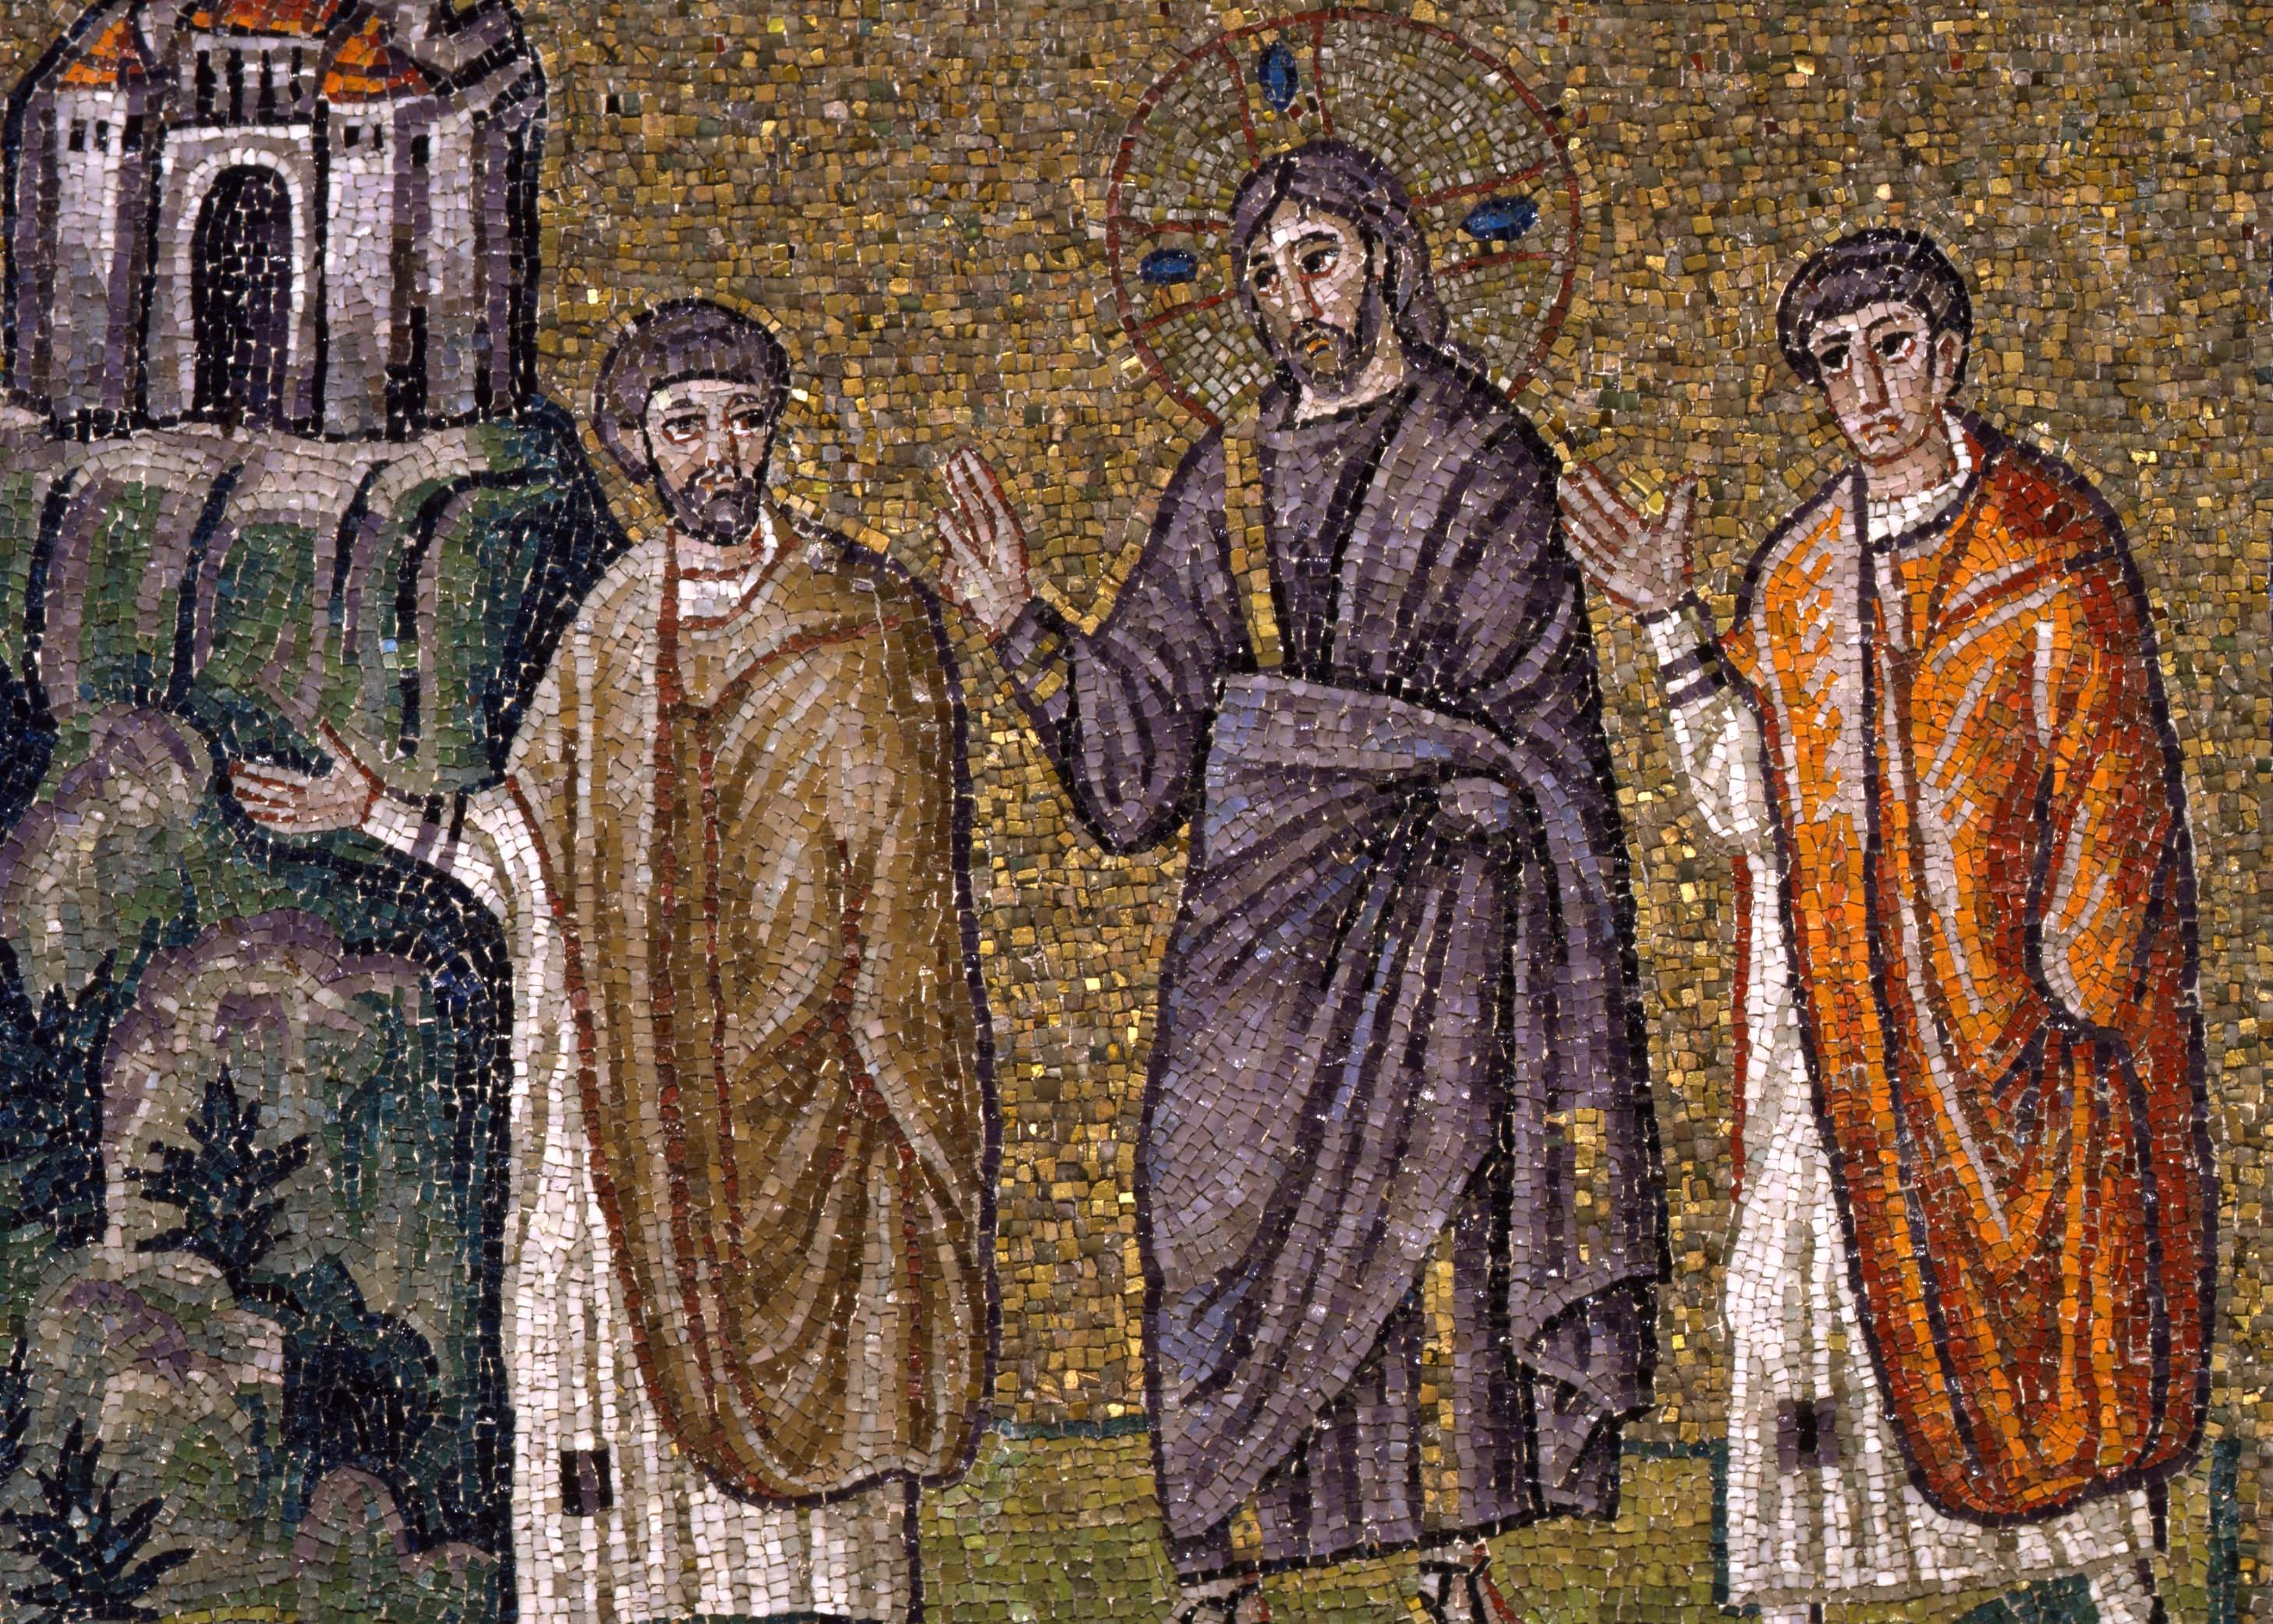
\includegraphics[width=8cm]{emmaus.jpg}
%\end{center}

\vfill

\begin{center}
%Ad usum et secundum consuetudines chori \guillemotright{}Conventus Choralis\guillemotleft.

%Editio Sancti Wolfgangi \annusEditionis
\end{center}

\pagebreak

\renewcommand{\headrulewidth}{0pt} % no horiz. rule at the header
\fancyhf{}
\pagestyle{fancy}

\cantusSineNeumas

\ifx\festumveldominica\undefined
\else
\pars{Oratio ante divinum Officium.}

\lettrine{{\color{red}A}}{peri,} Dómine, os meum ad benedicéndum nomen sanctum tuum:
munda quoque cor meum ab ómnibus vanis, pervérsis, et aliénis
cogitatiónibus:
intelléctum illúmina, afféctum inflámma,
ut digne, atténte ac devóte hoc Offícium recitáre váleam,
et exaudíri mérear ante conspéctum Divínæ Maiestátis tuæ.
Per Christum, Dóminum nostrum.
\Rbardot{} Amen.

Dómine, in unióne illíus divínæ intentiónis,
qua ipse in terris laudes Deo persolvísti,
has tibi Horas \rubricatum{(vel \textnormal{hanc tibi Horam})} persólvo.

%\trOratioAnteOfficium

\vfill

\pars{Oratio post divinum Officium.}

\rubrica{
  Orationem sequentem devote post Officium recitantibus
  Leo Papa X. defectus, et culpas in eo persolvendo ex humana
  fragilitate contractas, indulsit, et dicitur flexis genibus.
}

\lettrine{{\color{red}S}}{acrosánctæ} et indivíduæ Trinitáti,
crucifíxi Dómini nostri Iesu Christi humanitáti,
beatíssimæ et gloriosíssimæ sempérque Vírginis Maríæ
fecúndæ integritáti, 
et ómnium Sanctórum universitáti
sit sempitérna laus, honor, virtus et glória
ab omni creatúra,
nobísque remíssio ómnium peccatórum,
per infiníta sǽcula sæculórum.
\Rbardot{} Amen.

\noindent \Vbardot{} Beáta víscera Maríæ Virginis, quæ portavérunt
ætérni Patris Fílium.\\
\Rbardot{} Et beáta úbera, quæ lactavérunt Christum Dominum.

\rubrica{Et dicitur secreto \textnormal{Pater noster.} et \textnormal{Ave María.}}

%\trOratioPostOfficium

\vfill

\hora{Ad I. Vesperas.} %%%%%%%%%%%%%%%%%%%%%%%%%%%%%%%%%%%%%%%%%%%%%%%%%%%%%
%\sideThumbs{I. Vesperæ}

\vspace{0.5cm}
\grechangedim{interwordspacetext}{0.18 cm plus 0.15 cm minus 0.05 cm}{scalable}%
\ifx\festum\undefined
\cuminitiali{}{temporalia/deusinadiutorium-alter.gtex}
\else
\cuminitiali{}{temporalia/deusinadiutorium-solemnis.gtex}
\fi
\grechangedim{interwordspacetext}{0.22 cm plus 0.15 cm minus 0.05 cm}{scalable}%

\vfill
\pagebreak

\pars{Psalmus 1.} \scriptura{Ps. 109, 4; Gn. 14, 18}

\vspace{-0.4cm}

\antiphona{I f}{temporalia/ant-sacerdosinaeternum.gtex}

\scriptura{Psalmus 109.}

\initiumpsalmi{temporalia/ps109-initium-i-f-auto.gtex}

%\psalmusEtTranslatioT{temporalia/ps109-comb.tex}{10cm}
\input{temporalia/ps109.tex} \Abardot{}

\vspace{-1cm}

\vfill
\pagebreak

\vesperasi

\ifx\festum\undefined
\vesperasiii
\else
\vesperasii
\fi

\capitulumLaudes

% preklad Jeruz. bible
%\trCapituliI

\vfill

\ifx\dominica\undefined
\pars{Responsorium.} \scriptura{Ps. 30, 20; \textbf{H085}}

\cuminitiali{I}{temporalia/resp-quammagnamultitudo-cumdox.gtex}
\else
\pars{Responsorium breve.} \scriptura{Ps. 80, 17}

\cuminitiali{VI}{temporalia/resp-cibavit-simplex.gtex}
\fi

%\trResp

\vfill
\pagebreak

\vesperasiv

\ifx\dominica\undefined
\pars{Canticum B. Mariæ V.} \scriptura{Cf. Sap. 16, 21.20}

\vspace{-3mm}

{
\grechangedim{interwordspacetext}{0.18 cm plus 0.15 cm minus 0.05 cm}{scalable}%
\antiphona{VI F}{temporalia/ant-oquamsuavisest.gtex}
\grechangedim{interwordspacetext}{0.22 cm plus 0.15 cm minus 0.05 cm}{scalable}%
}

%\trAntIMagnificat

\vspace{-2mm}

\scriptura{Lc. 1, 46-55}

\vspace{-2mm}

\cantusSineNeumas
\initiumpsalmi{temporalia/magnificat-initium-visoll-F.gtex}

%\psalmusEtTranslatioT{temporalia/magnificat-I-comb.tex}{10.2cm}
\input{temporalia/magnificat-I.tex}

{
\grechangedim{interwordspacetext}{0.18 cm plus 0.15 cm minus 0.05 cm}{scalable}%
\antiphona{VI F}{temporalia/ant-oquamsuavisest.gtex}
\grechangedim{interwordspacetext}{0.22 cm plus 0.15 cm minus 0.05 cm}{scalable}%
}
\else
\pars{Canticum B. Mariæ V.} \scriptura{1 Sam. 3, 1; \textbf{B177v}}

\vspace{-3mm}

{
\grechangedim{interwordspacetext}{0.18 cm plus 0.15 cm minus 0.05 cm}{scalable}%
\antiphona{VII a}{temporalia/ant-puersamuelministrabat.gtex}
\grechangedim{interwordspacetext}{0.22 cm plus 0.15 cm minus 0.05 cm}{scalable}%
}

%\trAntIMagnificat

%\vspace{-3mm}

\scriptura{Lc. 1, 46-55}

%\vspace{-2mm}

\cantusSineNeumas
\initiumpsalmi{temporalia/magnificat-initium-viisoll-a.gtex}

%\vspace{-1.5mm}

%\psalmusEtTranslatioT{temporalia/magnificat-III-comb.tex}{10.2cm}
\input{temporalia/magnificat-III.tex} \Abardot{}
\fi

\vspace{-1cm}

\vfill
\pagebreak

%\sideThumbs{{\scriptsize{}Fine horarum}}

\anteOrationem

\pagebreak

% Oratio. %%%
\ifx\dominica\undefined
\cuminitiali{}{temporalia/oratio.gtex}
\else
\cuminitiali{}{temporalia/oratio2.gtex}
\fi

\vspace{-1mm}
%\trOrationisI

\vfill

\rubrica{Hebdomadarius dicit iterum Dominus vobiscum, vel cantor dicit:}

\vspace{2mm}

\sineinitiali{temporalia/domineexaudi.gtex}

\rubrica{Postea cantatur a cantore:}

\vspace{2mm}

\ifx\festum\undefined
\cuminitiali{II}{temporalia/benedicamus-semiduplex-vesp.gtex}
\else
\cuminitiali{II}{temporalia/benedicamus-solemnism-1vesp.gtex}
\fi

\vspace{1mm}

\vfill
\pagebreak
\fi

\ifx\festum\undefined
\else
\hora{Ad Completorium.} %%%%%%%%%%%%%%%%%%%%%%%%%%%%%%%%%%%%%%%%%%%%%%%%%%%%%%%%%%
%\sideThumbs{{\scriptsize{}Completorium}}

\rubrica{Lector petit benedictionem, dicens:}

\cuminitiali{}{temporalia/jubedomnebenedicere.gtex}

%\trJubeDomne

\vfill

\pars{Benedictio.}

\cuminitiali{}{temporalia/benedictio-noctemquietam.gtex}

%\trComplBenedictio

\vfill

\pars{Lectio brevis.} \scriptura{1Ptr. 5, 8-9}

\cuminitiali{}{temporalia/lectiobrevis-fratressobrii.gtex}

%\trComplLectioBr

\vfill

\noindent \Vbardot{} Adiutórium nostrum in nómine Dómini.

\noindent \Rbardot{} Qui fecit cælum, et terram.

\vfill
\pagebreak

\pars{Confessio.}

\noindent Confíteor Deo omnipoténti, beátæ Maríæ semper Vírgini, beáto
Michaéli Archángelo, beáto Ioánni Baptístæ, sanctis Apóstolis Petro
et Paulo, ómnibus Sanctis, et vobis fratres: quia peccávi nimis cogitatióne,
verbo et ópere: mea culpa, mea culpa, mea máxima culpa.
Ideo precor beátam Maríam semper Vírginem, beátum Michaélem
Archángelum, beátum Ioánnem Baptístam, sanctos Apóstolos Petrum
et Paulum, omnes Sanctos, et vos fratres, oráre pro me ad Dóminum
Deum nostrum.

\vfill

\noindent \Vbardot{} Misereátur nostri omnípotens Deus, et, dimíssis peccátis nostris, perdúcat
nos ad vitam ætérnam. \Rbardot{} Amen.

\vfill

\noindent \Vbardot{} Indulgéntiam, absolutiónem et remissiónem peccatórum nostrórum tríbuat nobis
omnípotens et miséricors Dóminus. \Rbardot{} Amen.

\vfill

\rubrica{Et facta absolutione dicitur:}

\sineinitiali{temporalia/convertenosdeus.gtex}

\vfill

\cuminitiali{}{temporalia/deusinadiutorium-communis.gtex}

\vfill
\pagebreak

\pars{Psalmus 1.}

\antiphona{VIII G}{temporalia/ant-miserere.gtex}

\scriptura{Ps. 4}

\initiumpsalmi{temporalia/ps4-initium-viii-G-auto.gtex}

%\psalmusEtTranslatioT{temporalia/ps4-comb.tex}{10cm}
\input{temporalia/ps4.tex}

\vfill
\pagebreak

\pars{Psalmus 2.} \scriptura{Ps. 90}

\initiumpsalmi{temporalia/ps90-initium-viii-G-auto.gtex}

%\psalmusEtTranslatioT{temporalia/ps90-comb.tex}{10cm}
\input{temporalia/ps90.tex}

\pagebreak

\pars{Psalmus 3.} \scriptura{Ps. 133}

\initiumpsalmi{temporalia/ps133-initium-viii-G-auto.gtex}

%\psalmusEtTranslatioT{temporalia/ps133-comb.tex}{10cm}
\input{temporalia/ps133.tex}

\vfill

\antiphona{}{temporalia/ant-miserere.gtex}

\vfill

\pars{Hymnus.}

\antiphona{II}{temporalia/hym-TeLucis.gtex}
%\begin{translatioMulticol}{3}
Než světlo zhasne prosíme\\
Tebe tvůrce všech pokorně,\\
abys nám ve své milosti\\
byl ochranou a~pomocí.\columnbreak

Ať vzdáleny jsou od nás sny\\
a~těžké noční přízraky.\\
Zdrť našeho nepřítele,\\
těla poskvrn ať ujdeme.\columnbreak

Tobě buď sláva, Ježíši,\\
národům že ses projevil,\\
Otci i~Duchu života\\
po věkoucí věky světa.\\
Amen.
\end{translatioMulticol}


\pagebreak

\pars{Capitulum.} \scriptura{Ier. 14, 9}

\cuminitiali{}{temporalia/capitulum-tuautem.gtex}

% preklad Jeruz. bible
%\trComplCapituli

\vfill

\pars{Responsorium breve.} \scriptura{Ps. 30, 6}

\cuminitiali{VI}{temporalia/resp-inmanus.gtex}

%\trRespCompl
\vfill

\pars{Versus.} \scriptura{Ps. 16, 8}

\sineinitiali{temporalia/versus-custodi.gtex}

%\noindent \trComplVersus

\vfill
\pagebreak

\cantusCumNeumis

\pars{Canticum Simeonis.}

\vspace{-3mm}

\antiphona{III a}{temporalia/ant-salvanos-antiquo.gtex}

%\trAntSalvaNos

%\vspace{-1mm}

\scriptura{Lc. 2, 29-32}

\vspace{-2mm}

\initiumpsalmi{temporalia/nuncdimittis-initium-iii-a-auto.gtex}

%\psalmusEtTranslatioT{temporalia/nuncdimittis-comb.tex}{10cm}
\input{temporalia/nuncdimittis.tex} \Abardot{}

\vfill

\rubrica{Ante Orationem, cantatur a Superiore:}

\vspace{3mm}

\pars{Supplicatio Litaniæ.}

\cuminitiali{}{temporalia/supplicatiolitaniae.gtex}

\vspace{7mm}

\pars{Oratio Dominica.}

\noindent Pater noster.

\vfill
\pagebreak

\sineinitiali{temporalia/domineexaudi-simplex.gtex}

\vspace{7mm}

\pars{Oratio.}

\cantusSineNeumas

\cuminitiali{}{temporalia/oratio-visita.gtex}

%\trComplOrationis

\vfill

%\sineinitiali{temporalia/domineexaudi-communis.gtex}

\noindent \Vbardot{} Dómine, exáudi oratiónem meam. \Rbardot{} Et clamor meus ad te véniat.

\vfill

%\vfill

\sineinitiali{temporalia/benedicamus-minor.gtex}

\vfill

\pars{Benedictio.}

\noindent Benedícat et custódiat nos omnípotens et miséricors Dóminus, \gredagger{}
Pater, et Fílius, et Spíritus Sanctus. \Rbardot{} Amen.

\vfill
\pagebreak

\pars{Antiphona finalis B. M. V.}

\vspace{-4mm}

\antiphona{I}{temporalia/an_salve_regina.gtex}

\rubrica{vel:}

\vspace{-4mm}

\antiphona{V}{temporalia/ant-salveregina-simplex.gtex}

\vfill
\pagebreak

\rubrica{vel:}

\antiphona{VII}{temporalia/ant-subtuum.gtex}

\vfill
\pagebreak
\fi

\hora{Ad Matutinum.} %%%%%%%%%%%%%%%%%%%%%%%%%%%%%%%%%%%%%%%%%%%%%%%%%%%%%
%\sideThumbs{Matutinum}

\vspace{2mm}

\cuminitiali{}{temporalia/dominelabiamea.gtex}

\vspace{2mm}

\pars{Invitatorium.} \scriptura{Cantor; \textbf{LU\textsubscript{918}}}

\vspace{-6mm}

\antiphona{IV}{temporalia/inv-christumregemadoremus.gtex}

\vfill
\pagebreak

\pars{Hymnus.}

\vspace{-5mm}

\scriptura{Thomas de Aquino; \textbf{LU\textsubscript{920}}}

\antiphona{IV}{temporalia/hym-SacrisSolemniis.gtex}
%{
%\vspace{-5mm}
%\setlength{\columnsep}{0pt} % prostor mezi sloupci
%\input{hym-SacrisSolemniis-bohtext.tex}
%\setlength{\columnsep}{30pt} % prostor mezi sloupci
%}

\vfill
\pagebreak

\subhora{In I. Nocturno}

\pars{Psalmus 1.} \scriptura{Ps. 1, 3; \textbf{LU\textsubscript{922}}}

\vspace{-2mm}

\antiphona{I D*}{temporalia/ant-fructumsalutiferum.gtex}

%\vspace{-5mm}

\scriptura{Ps. 1}

%\vspace{-2mm}

\initiumpsalmi{temporalia/ps1-initium-i-D_-auto.gtex}

%\psalmusEtTranslatioT{temporalia/ps1-comb.tex}{10cm}
\input{temporalia/ps1.tex} \Abardot{}

\vfill
\pagebreak

\pars{Psalmus 2.} \scriptura{Ps. 4, 8.9; \textbf{LU\textsubscript{923}}}

\vspace{-2mm}

\antiphona{II D}{temporalia/ant-afructufrumenti.gtex}

%\vspace{-5mm}

\scriptura{Ps. 4}

\initiumpsalmi{temporalia/ps4-initium-ii-D-auto.gtex}

%\psalmusEtTranslatioT{temporalia/ps4iiD-comb.tex}{10cm}
\input{temporalia/ps4iiD.tex} \Abardot{}

\vfill
\pagebreak

\pars{Psalmus 3.} \scriptura{Ps. 15, 4; \textbf{LU\textsubscript{924}}}

\vspace{-4mm}

\antiphona{III a\textsuperscript{3}}{temporalia/ant-communionecalicis.gtex}

%\vspace{-2mm}

\scriptura{Ps. 15}

\vspace{-2mm}

\initiumpsalmi{temporalia/ps15-initium-iii-a3-auto.gtex}

%\psalmusEtTranslatioT{temporalia/ps15-comb.tex}{10cm}
\input{temporalia/ps15.tex} \Abardot{}

\vfill
\pagebreak

\pars{Versus.} \scriptura{Sap. 16, 20; Ps. 77, 25}

% Versus. %%%
\sineinitiali{temporalia/versus-panemdecaelohomo-communis.gtex}

\vspace{5mm}

\sineinitiali{temporalia/oratiodominica-mat.gtex}

\vspace{5mm}

\pars{Absolutio.}

\cuminitiali{}{temporalia/absolutio-exaudi.gtex}

\vfill
\pagebreak

\cuminitiali{}{temporalia/benedictio-solemn-benedictione.gtex}

\vspace{7mm}

\lectioi

\noindent \Vbardot{} Tu autem, Dómine, miserére nobis.
\noindent \Rbardot{} Deo grátias.

\vfill
\pagebreak

\pars{Responsorium 1.} \scriptura{\Rbardot{} Ex. 12, 5.6.8 \Vbardot{} 1 Cor. 5, 7.8; \textbf{LU\textsubscript{926}}}

\vspace{-2mm}

\responsorium{I}{temporalia/resp-immolabithaedum.gtex}{}

\vfill
\pagebreak

\cuminitiali{}{temporalia/benedictio-solemn-unigenitus.gtex}

\vspace{7mm}

\lectioii

\noindent \Vbardot{} Tu autem, Dómine, miserére nobis.
\noindent \Rbardot{} Deo grátias.

\vfill
\pagebreak

\pars{Responsorium 2.} \scriptura{\Rbardot{} Ex. 16, 12.15 \Vbardot{} Io. 6, 21; \textbf{LU\textsubscript{927}}}

\vspace{-2mm}

\responsorium{II}{temporalia/resp-comedetiscarnes.gtex}{}

\vfill
\pagebreak

\cuminitiali{}{temporalia/benedictio-solemn-spiritus.gtex}

\vspace{7mm}

\lectioiii

\noindent \Vbardot{} Tu autem, Dómine, miserére nobis.
\noindent \Rbardot{} Deo grátias.

\vfill
\pagebreak

\pars{Responsorium 3.} \scriptura{\Rbardot{} 3 Reg. 19, 6.8 \Vbardot{} Io. 6, 52; \textbf{LU\textsubscript{927}}}

\vspace{-2mm}

\responsorium{III}{temporalia/resp-respexitelias.gtex}{}

\vfill
\pagebreak

\subhora{In II. Nocturno}

\pars{Psalmus 4.} \scriptura{Ps. 19, 4; \textbf{LU\textsubscript{928}}}

\vspace{-2mm}

\antiphona{IV E}{temporalia/ant-memorsit-FKP.gtex}

\vspace{-2mm}

\scriptura{Ps. 19}

\initiumpsalmi{temporalia/ps19-initium-iv-E-auto.gtex}

%\psalmusEtTranslatioT{temporalia/ps19-comb.tex}{10cm}
\input{temporalia/ps19.tex} \Abardot{}

\vfill
\pagebreak

\pars{Psalmus 5.} \scriptura{Ps. 22, 5; \textbf{LU\textsubscript{928}}}

\vspace{-2mm}

\antiphona{V a}{temporalia/ant-paraturnobis-FKP.gtex}

%\vspace{-3mm}

\scriptura{Ps. 22}

%\vspace{-2mm}

\initiumpsalmi{temporalia/ps22-initium-v-a.gtex}

%\vspace{-1.5mm}

%\psalmusEtTranslatioT{temporalia/ps22-comb.tex}{10cm}
\input{temporalia/ps22.tex} \Abardot{}

\vspace{-1cm}

\vfill
\pagebreak

\pars{Psalmus 6.} \scriptura{Ps. 41, 5; \textbf{LU\textsubscript{930}}}

\vspace{-2mm}

\antiphona{VI F}{temporalia/ant-invoceexsultationis-FKP.gtex}

%\vspace{-5mm}

\scriptura{Ps. 41}

\initiumpsalmi{temporalia/ps41-initium-vi-F-auto.gtex}

%\psalmusEtTranslatioT{temporalia/ps41-comb.tex}{10cm}
\input{temporalia/ps41.tex}

\vfill

\antiphona{}{temporalia/ant-invoceexsultationis-FKP.gtex}

\vfill
\pagebreak

\pars{Versus.} \scriptura{Ps. 80, 17}

% Versus. %%%
\sineinitiali{temporalia/versus-cibavit.gtex}

\vspace{5mm}

\sineinitiali{temporalia/oratiodominica-mat.gtex}

\vspace{5mm}

\pars{Absolutio.}

\cuminitiali{}{temporalia/absolutio-ipsius.gtex}

\vfill
\pagebreak

\cuminitiali{}{temporalia/benedictio-solemn-deus.gtex}

\vspace{7mm}

\lectioiv

\noindent \Vbardot{} Tu autem, Dómine, miserére nobis.
\noindent \Rbardot{} Deo grátias.

\vfill
\pagebreak

\pars{Responsorium 4.} \scriptura{\Rbardot{} Mt. 26, 26 \Vbardot{} Io. 31, 31; \textbf{LU\textsubscript{931}}}

\vspace{-2mm}

\responsorium{V}{temporalia/resp-coenantibus.gtex}{}

\vfill
\pagebreak

\cuminitiali{}{temporalia/benedictio-solemn-christus.gtex}

\vspace{7mm}

\lectiov

\noindent \Vbardot{} Tu autem, Dómine, miserére nobis.
\noindent \Rbardot{} Deo grátias.

\vfill
\pagebreak

\pars{Responsorium 5.} \scriptura{\Rbardot{} 1 Cor. 11, 25 \Vbardot{} Thren. 3, 20; \textbf{LU\textsubscript{932}}}

\vspace{-2mm}

\responsorium{VI}{temporalia/resp-accepitiesus.gtex}{}

\vfill
\pagebreak

\cuminitiali{}{temporalia/benedictio-solemn-ignem.gtex}

\vspace{7mm}

\lectiovi

\noindent \Vbardot{} Tu autem, Dómine, miserére nobis.
\noindent \Rbardot{} Deo grátias.

\vfill
\pagebreak

\pars{Responsorium 6.} \scriptura{\Rbardot{} Io. 6, 48 \Vbardot{} ibid. 6, 51.52; \textbf{LU\textsubscript{934}}}

\vspace{-2mm}

\responsorium{VII}{temporalia/resp-egosumpanisvitae.gtex}{}

\vfill
\pagebreak

\subhora{In III. Nocturno}

\pars{Psalmus 7.} \scriptura{Ps. 42, 4; \textbf{LU\textsubscript{934}}}

\vspace{-5mm}

\antiphona{VII a}{temporalia/ant-introibo-FKP.gtex}

\vspace{-4mm}

\scriptura{Ps. 42}

%\vspace{-2mm}

\initiumpsalmi{temporalia/ps42-initium-vii-a-auto.gtex}

%\psalmusEtTranslatioT{temporalia/ps42-comb.tex}{10cm}
\input{temporalia/ps42.tex} \Abardot{}

\vfill
\pagebreak

\pars{Psalmus 8.} \scriptura{Ps. 80, 17; \textbf{LU\textsubscript{935}}}

\vspace{-5mm}

\antiphona{VIII G}{temporalia/ant-cibavitnos-FKP.gtex}

\vspace{-3mm}

\scriptura{Ps. 80}

\vspace{-2mm}

\initiumpsalmi{temporalia/ps80-initium-viii-G-auto.gtex}

\vspace{-1mm}

%\psalmusEtTranslatioT{temporalia/ps80-comb.tex}{10cm}
\input{temporalia/ps80.tex} \Abardot{}

\vfill
\pagebreak

\pars{Psalmus 9.} \scriptura{Ps. 83, 3; \textbf{LU\textsubscript{936}}}

\vspace{-2mm}

\antiphona{VI F}{temporalia/ant-exaltari-FKP.gtex}

\vspace{-2mm}

\scriptura{Ps. 83}

\initiumpsalmi{temporalia/ps83-initium-vi-F-auto.gtex}

%\psalmusEtTranslatioT{temporalia/ps83-comb.tex}{10cm}
\input{temporalia/ps83.tex} \Abardot{}

\vfill
\pagebreak

\pars{Versus.} \scriptura{Ps. 103, 14-15}

% Versus. %%%
\sineinitiali{temporalia/versus-educas.gtex}

\vspace{5mm}

\sineinitiali{temporalia/oratiodominica-mat.gtex}

\vspace{5mm}

\pars{Absolutio.}

\cuminitiali{}{temporalia/absolutio-avinculis.gtex}

\vfill
\pagebreak

\cuminitiali{}{temporalia/benedictio-solemn-evangelica.gtex}

\vspace{7mm}

\lectiovii

\noindent \Vbardot{} Tu autem, Dómine, miserére nobis.
\noindent \Rbardot{} Deo grátias.

\vfill
\pagebreak

\pars{Responsorium 7.} \scriptura{\Rbardot{} Io. 6, 57 \Vbardot{} Dt. 4, 7; \textbf{LU\textsubscript{938}}}

\vspace{-2mm}

\responsorium{VII}{temporalia/resp-quimanducat.gtex}{}

\vfill
\pagebreak

\cuminitiali{}{temporalia/benedictio-solemn-divinum.gtex}

\vspace{7mm}

\lectioviii

\noindent \Vbardot{} Tu autem, Dómine, miserére nobis.
\noindent \Rbardot{} Deo grátias.

\vfill
\pagebreak

\ifx\dominica\undefined
\pars{Responsorium 8.} \scriptura{\Rbardot{} Io. 6, 58 \Vbardot{} Eccli. 15, 3; \textbf{LU\textsubscript{938}}}

\vspace{-2mm}

\responsorium{VIII}{temporalia/resp-misitmevivenspater.gtex}{}
\else
\pars{Responsorium 8.} \scriptura{\Rbardot{} Lc. 14, 16-17 \Vbardot{} Prv. 9, 5}

\vspace{-2mm}

\responsorium{VI}{temporalia/resp-homoquidamfecit.gtex}{}
\fi

\vfill
\pagebreak

\cuminitiali{}{temporalia/benedictio-solemn-adsocietatem.gtex}

\vspace{7mm}

\lectioix

\noindent \Vbardot{} Tu autem, Dómine, miserére nobis.
\noindent \Rbardot{} Deo grátias.

\vfill
\pagebreak

% Te Deum

%\pars{Hymnus Ambrosianus}

\vspace{-5mm}

\ifx\solemnis\undefined
\ifx\aequus\undefined
{
\pars{Hymnus Ambrosianus} \scriptura{Alio modo, iuxta morem Romanum}

\vspace{-2mm}

\grechangedim{interwordspacetext}{0.26 cm plus 0.15 cm minus 0.05 cm}{scalable}%
\cuminitiali{III}{temporalia/tedeum-romanum-gn.gtex}
\grechangedim{interwordspacetext}{0.22 cm plus 0.15 cm minus 0.05 cm}{scalable}%
}
\else
{
\pars{Hymnus Ambrosianus} \scriptura{Tonus Simplex}

\vspace{-2mm}

\grechangedim{interwordspacetext}{0.30 cm plus 0.15 cm minus 0.05 cm}{scalable}%
\cuminitiali{III}{temporalia/tedeum-simplex-gn.gtex}
\grechangedim{interwordspacetext}{0.22 cm plus 0.15 cm minus 0.05 cm}{scalable}%
}
\fi
\else
{
\pars{Hymnus Ambrosianus} \scriptura{Tonus Solemnis}

\vspace{-2mm}

\grechangedim{interwordspacetext}{0.26 cm plus 0.15 cm minus 0.05 cm}{scalable}%
\cuminitiali{III}{temporalia/tedeum-solemnis-gn.gtex}
\grechangedim{interwordspacetext}{0.22 cm plus 0.15 cm minus 0.05 cm}{scalable}%
}
\fi

\vfill
\pagebreak

\rubrica{Reliqua omittuntur, nisi Laudes separandæ sint.}

\sineinitiali{temporalia/domineexaudi.gtex}

\vfill

\pars{Oratio.}

\ifx\dominica\undefined
\cuminitiali{}{temporalia/oratio.gtex}
\else
\cuminitiali{}{temporalia/oratio2.gtex}
\fi

\vfill

\noindent \Vbardot{} Dómine, exáudi oratiónem meam.
\Rbardot{} Et clamor meus ad te véniat.

\vfill

% Nocturnale Romanum 2002, p. LXXVI Benedicamus Domino seems to match
% the one from Solemn Laudes.
\cuminitiali{V}{temporalia/benedicamus-solemnis-laud.gtex}

\vfill

\noindent \Vbardot{} Fidélium ánimæ per misericórdiam Dei requiéscant in pace.
\Rbardot{} Amen.

\vfill
\pagebreak

\hora{Ad Laudes.} %%%%%%%%%%%%%%%%%%%%%%%%%%%%%%%%%%%%%%%%%%%%%%%%%%%%%
%\sideThumbs{Laudes}

\cantusSineNeumas

\vspace{0.5cm}
\grechangedim{interwordspacetext}{0.18 cm plus 0.15 cm minus 0.05 cm}{scalable}%
\ifx\festumveldominica\undefined
\cuminitiali{}{temporalia/deusinadiutorium-communis.gtex}
\else
\cuminitiali{}{temporalia/deusinadiutorium-alter.gtex}
\fi
\grechangedim{interwordspacetext}{0.22 cm plus 0.15 cm minus 0.05 cm}{scalable}%

\vfill
%\pagebreak

\pars{Psalmus 1.} \scriptura{Prv. 9, 1-2}

\vspace{-0.4cm}

\antiphona{I a\textsuperscript{2}}{temporalia/ant-sapientiaaedificavit.gtex}

\scriptura{Psalmus 92.}

\initiumpsalmi{temporalia/ps92-initium-i-a2-auto.gtex}

%\psalmusEtTranslatioT{temporalia/ps92-comb.tex}{10cm}
\input{temporalia/ps92.tex} \Abardot{}

\vfill
\pagebreak

\pars{Psalmus 2.} \scriptura{Sap. 16, 20}

\vspace{-0.4cm}

\antiphona{II D}{temporalia/ant-angelorumesca.gtex}

\scriptura{Psalmus 99.}

\initiumpsalmi{temporalia/ps99-initium-ii-D-auto.gtex}

%\psalmusEtTranslatioT{temporalia/ps99-comb.tex}{10cm}
\input{temporalia/ps99.tex} \Abardot{}

\vfill
\pagebreak

\pars{Psalmus 3.} \scriptura{Gn. 48, 20}

\vspace{-0.4cm}

\antiphona{III a}{temporalia/ant-pinguisest.gtex}

\scriptura{Psalmus 62.}

\initiumpsalmi{temporalia/ps62-initium-iii-a-auto.gtex}

%\psalmusEtTranslatioT{temporalia/ps62-comb.tex}{10cm}
\input{temporalia/ps62.tex} \Abardot{}

\vfill
\pagebreak

\pars{Psalmus 4.} \scriptura{Cf. Lv. 21, 6}

\vspace{-0.4cm}

\antiphona{IV E}{temporalia/ant-sacerdotessancti.gtex}

\scriptura{Canticum trium puerorum, Dan. 3, 57-88 et 56}

\initiumpsalmi{temporalia/dan3-initium-iv-E-auto.gtex}

%\psalmusEtTranslatioT{temporalia/dan3-comb.tex}{10cm}
\input{temporalia/dan3.tex}

\rubrica{Hic non dicitur Gloria Patri, neque Amen.}

\vfill

\vspace{-6mm}

\antiphona{}{temporalia/ant-sacerdotessancti.gtex} % repeat the antiphon - new page

\vfill
\pagebreak

\pars{Psalmus 5.} \scriptura{Ap. 2, 17}

\vspace{-0.4cm}

\antiphona{V a}{temporalia/ant-vincentidabo.gtex}

\scriptura{Psalmus 148.}

\initiumpsalmi{temporalia/ps148-initium-v-a-auto.gtex}

%\psalmusEtTranslatioT{temporalia/ps148-comb.tex}{10cm}
\input{temporalia/ps148.tex}

\rubrica{Hic non dicitur Gloria Patri.}

\vfill
\pagebreak

%
\scriptura{Psalmus 149.}

\initiumpsalmi{temporalia/ps149-initium-v-a-auto.gtex}

%\psalmusEtTranslatioT{temporalia/ps149-comb.tex}{10cm}
\input{temporalia/ps149.tex}

\rubrica{Hic non dicitur Gloria Patri.}

\vfill
\pagebreak

%
\scriptura{Psalmus 150.}

\initiumpsalmi{temporalia/ps150-initium-v-a-auto.gtex}

%\psalmusEtTranslatioT{temporalia/ps150-comb.tex}{10cm}
\input{temporalia/ps150.tex}

\vfill

\vspace{-6mm}

\antiphona{}{temporalia/ant-vincentidabo.gtex} % repeat the antiphon - new page

\vfill
\pagebreak

\capitulumLaudes

% preklad Jeruz. bible
%\trCapituliI

\vfill

\pars{Responsorium breve.} \scriptura{Ps. 77, 24-25}

\cuminitiali{VI}{temporalia/resp-panemcaeli.gtex}

%\trResp

\vfill
\pagebreak

\pars{Hymnus} \scriptura{Thomas de Aquino?}

\cuminitiali{VIII}{temporalia/hym-VerbumSupernum.gtex}
\vspace{-3mm}
%\begin{translatioMulticol}{5}
Nebeské Slovo, Syn ty jsi\\
a světlo z Otce prýštící,\\
jenž zrozen, jdeš zachránit svět,\\
když naplnil se časů věk.\columnbreak

Už teď nám duši rozjasni\\
a plamen lásky zapal v ní,\\
ať srdce vlády zbavené\\
nebeská rozkoš naplní.\columnbreak

Aby, až soudce na trůnu\\
ohni zlé bude vydávat\\
a ty, kdo toho hodni jsou,\\
milý hlas v nebe povolá,\columnbreak

zmatku temnot ať vydáni\\
nejsme, ni v stravu plamenů,\\
leč na tvář Boha pohledět\\
smíme a těšit se v nebesích.\columnbreak

Otci společně se Synem,\\
a Tobě, Duše přesvatý,\\
sláva, jež vždycky trvala,\\
stejná budiž i na věky.\\
Amen.
\end{translatioMulticol}


\vfill
%\pagebreak

\pars{Versus.} \scriptura{Ps. 147, 3}

% Versus. %%%
\ifx\festum\undefined
\sineinitiali{temporalia/versus-posuitfines-communis.gtex}
\else
\sineinitiali{temporalia/versus-posuitfines.gtex}
\fi

%\noindent \trVersus

\vfill
\pagebreak

\ifx\dominica\undefined
\pars{Canticum Zachariæ.} \scriptura{Io. 6, 51.52}

\vspace{-4mm}

{
\grechangedim{interwordspacetext}{0.18 cm plus 0.15 cm minus 0.05 cm}{scalable}%
\antiphona{I a\textsuperscript{2}}{temporalia/ant-egosumpanisvivus.gtex}
\grechangedim{interwordspacetext}{0.22 cm plus 0.15 cm minus 0.05 cm}{scalable}%
}

%\trAntIMagnificat

\vspace{-2mm}

\scriptura{Lc. 1, 68-79}

\vspace{-1mm}

\cantusSineNeumas
\ifx\solemnis\undefined
\initiumpsalmi{temporalia/benedictus-initium-i-a2-auto.gtex}

%\vspace{-1.5mm}

%\psalmusEtTranslatioT{temporalia/benedictus-III-comb.tex}{10.2cm}
\input{temporalia/benedictus-III.tex} \Abardot{}
\else
\initiumpsalmi{temporalia/benedictus-initium-isoll-a2-auto.gtex}

%\vspace{-1.5mm}

%\psalmusEtTranslatioT{temporalia/benedictus-I-comb.tex}{10.2cm}
\input{temporalia/benedictus-I.tex} \Abardot{}
\fi
\else
\pars{Canticum Zachariæ.} \scriptura{Lc. 14, 16.17}

\vspace{-4mm}

{
\grechangedim{interwordspacetext}{0.18 cm plus 0.15 cm minus 0.05 cm}{scalable}%
\antiphona{III g\textsuperscript{2}}{temporalia/ant-homoquidam.gtex}
\grechangedim{interwordspacetext}{0.22 cm plus 0.15 cm minus 0.05 cm}{scalable}%
}

%\trAntIMagnificat

\vspace{-2mm}

\scriptura{Lc. 1, 68-79}

\vspace{-2mm}

\cantusSineNeumas
\initiumpsalmi{temporalia/benedictus-initium-iiisoll-g2-auto.gtex}

%\vspace{-1mm}

%\psalmusEtTranslatioT{temporalia/benedictus-II-comb.tex}{10.2cm}
\input{temporalia/benedictus-II.tex} \Abardot{}
\fi

\vspace{-1cm}

\vfill
\pagebreak

%\sideThumbs{{\scriptsize{}Fine horarum}}

\anteOrationem

\pagebreak

% Oratio. %%%
\ifx\dominica\undefined
\cuminitiali{}{temporalia/oratio.gtex}
\else
\cuminitiali{}{temporalia/oratio2.gtex}
\fi

\vspace{-1mm}
%\trOrationisI

\vfill

\rubrica{Hebdomadarius dicit iterum Dominus vobiscum, vel cantor dicit:}

\vspace{2mm}

\sineinitiali{temporalia/domineexaudi.gtex}

\rubrica{Postea cantatur a cantore:}

\vspace{2mm}

\ifx\festum\undefined
\ifx\octava\undefined
\cuminitiali{I}{temporalia/benedicamus-semiduplex-laud.gtex}
\else
\cuminitiali{VIII}{temporalia/benedicamus-duplexmajus-laudes.gtex}
\fi
\else
\cuminitiali{II}{temporalia/benedicamus-solemnism-laud.gtex}
\fi

\vspace{1mm}

\vfill
\pagebreak

\ifx\sabbatoveloctava\undefined
\ifx\festumveldominica\undefined
\hora{Ad Vesperas.} %%%%%%%%%%%%%%%%%%%%%%%%%%%%%%%%%%%%%%%%%%%%%%%%%%%%%
%\sideThumbs{Vesperæ}
\else
\hora{Ad II. Vesperas.} %%%%%%%%%%%%%%%%%%%%%%%%%%%%%%%%%%%%%%%%%%%%%%%%%%%%%
%\sideThumbs{II. Vesperæ}
\fi

\cantusSineNeumas

%\vspace{-2mm}
\grechangedim{interwordspacetext}{0.18 cm plus 0.15 cm minus 0.05 cm}{scalable}%
\ifx\festumveldominica\undefined
\cuminitiali{}{temporalia/deusinadiutorium-communis.gtex}
\else
\ifx\festum\undefined
\cuminitiali{}{temporalia/deusinadiutorium-alter.gtex}
\else
\cuminitiali{}{temporalia/deusinadiutorium-solemnis.gtex}
\fi
\fi
\grechangedim{interwordspacetext}{0.22 cm plus 0.15 cm minus 0.05 cm}{scalable}%

\vfill
%\pagebreak

%\vspace{-2mm}

\pars{Psalmus 1.} \scriptura{Ps. 109, 4; Gn. 14, 18}

\vspace{-0.4cm}

\antiphona{I f}{temporalia/ant-sacerdosinaeternum.gtex}

\scriptura{Psalmus 109.}

\initiumpsalmi{temporalia/ps109-initium-i-f-auto.gtex}

%\psalmusEtTranslatioT{temporalia/ps109-comb.tex}{10cm}
\input{temporalia/ps109.tex} \Abardot{}

%\vfill

%\antiphona{}{temporalia/ant-sacerdosinaeternum.gtex}

%\vspace{-1cm}

\vfill
\pagebreak

\vesperasi

\ifx\aequus\undefined
\vesperasii
\else
\vesperasiii
\fi

\capitulumLaudes

% preklad Jeruz. bible
%\trCapituliI

\vfill

\pars{Responsorium breve.} \scriptura{Ps. 80, 17}

\ifx\festum\undefined
\cuminitiali{VI}{temporalia/resp-cibavit-simplex.gtex}
\else
\cuminitiali{VI}{temporalia/resp-cibavit.gtex}
\fi

%\trResp

\vfill
\pagebreak

\vesperasiv

\ifx\dominica\undefined
\pars{Canticum B. Mariæ V.} \scriptura{Thomas de Aquino?}

%\vspace{-5.5mm}

{
\grechangedim{interwordspacetext}{0.18 cm plus 0.15 cm minus 0.05 cm}{scalable}%
\antiphona{V a}{temporalia/ant-osacrumconvivium.gtex}
\grechangedim{interwordspacetext}{0.22 cm plus 0.15 cm minus 0.05 cm}{scalable}%
}

%\trAntIMagnificat

\vspace{-3mm}

\scriptura{Lc. 1, 46-55}

\vspace{-2.5mm}

\cantusSineNeumas
\ifx\solemnis\undefined
\initiumpsalmi{temporalia/magnificat-initium-v-a_.gtex}

\vspace{-1.5mm}

%\psalmusEtTranslatioT{temporalia/magnificat-V-comb.tex}{10.2cm}
\input{temporalia/magnificat-V.tex} \Abardot{}
\else
\initiumpsalmi{temporalia/magnificat-initium-vsoll-a_.gtex}

\vspace{-1.5mm}

%\psalmusEtTranslatioT{temporalia/magnificat-II-comb.tex}{10.2cm}
\input{temporalia/magnificat-II.tex} \Abardot{}
\fi
\else
\pars{Canticum B. Mariæ V.} \scriptura{Lc. 14, 21.23; \textbf{H427}}

\vspace{-6mm}

{
\grechangedim{interwordspacetext}{0.18 cm plus 0.15 cm minus 0.05 cm}{scalable}%
\antiphona{I a}{temporalia/ant-exicitoinplateas.gtex}
\grechangedim{interwordspacetext}{0.22 cm plus 0.15 cm minus 0.05 cm}{scalable}%
}

\vspace{-2mm}

%\trAntIMagnificat

\scriptura{Lc. 1, 46-55}

\vspace{-2mm}

\cantusSineNeumas
\initiumpsalmi{temporalia/magnificat-initium-isoll-a.gtex}

\vspace{-1mm}

%\psalmusEtTranslatioT{temporalia/magnificat-IV-comb.tex}{10.2cm}
\input{temporalia/magnificat-IV.tex} \Abardot{}
\fi

\vspace{-1cm}

\vfill
\pagebreak

%\sideThumbs{{\scriptsize{}Fine horarum}}

\anteOrationem

\pagebreak

% Oratio. %%%
\ifx\dominica\undefined
\cuminitiali{}{temporalia/oratio.gtex}
\else
\cuminitiali{}{temporalia/oratio2.gtex}
\fi

\vspace{-1mm}
%\trOrationisI

\vfill

\rubrica{Hebdomadarius dicit iterum Dominus vobiscum, vel cantor dicit:}

\vspace{2mm}

\sineinitiali{temporalia/domineexaudi.gtex}

\rubrica{Postea cantatur a cantore:}

\vspace{2mm}

\ifx\festum\undefined
\cuminitiali{II}{temporalia/benedicamus-semiduplex-vesp.gtex}
\else
\cuminitiali{II}{temporalia/benedicamus-solemnism-2vesp.gtex}
\fi

\vspace{1mm}
\fi

\end{document}

